%%%%%%%%%%%%%%%%%%%%%%%%%%%%%%%%%%%%%%%%%%  不使用 authblk 包制作标题  %%%%%%%%%%%%%%%%%%%%%%%%%%%%%%%%%%%%%%%%%%%%%%
%-------------------------------PPT Title-------------------------------------
\title{\rm{VASP}软件:~\rm{PAW}方法、并行、迭代优化和赝势}
%-----------------------------------------------------------------------------

%----------------------------Author & Date------------------------------------
\author[\textrm{Jun\_Jiang}]{姜\;\;骏\inst{}} %[]{} (optional, use only with lots of authors)
%% - Give the names in the same order as the appear in the paper.
%% - Use the \inst{?} command only if the authors have different
%%   affiliation.
\institute[BCC]{\inst{}%
%\institute[Gain~Strong]{\inst{}%
\vskip -20pt 北京市计算中心}
%\vskip -20pt {\large 格致斯创~科技}}
\date[\today] % (optional, should be abbreviation of conference name)
{	{\fontsize{6.2pt}{4.2pt}\selectfont{\textcolor{blue}{E-mail:~}\url{jiangjun@bcc.ac.cn}}}
\vskip 45 pt {\fontsize{8.2pt}{6.2pt}\selectfont{%清华大学\;\;物理系% 报告地点
	\vskip 5 pt \textrm{2023.07.05}}}
}

%% - Either use conference name or its abbreviation
%% - Not really information to the audience, more for people (including
%%   yourself) who are reading the slides onlin%%   yourself) who are reading the slides onlin%%   yourself) who are reading the slides onlineee
%%%%%%%%%%%%%%%%%%%%%%%%%%%%%%%%%%%%%%%%%%%%%%%%%%%%%%%%%%%%%%%%%%%%%%%%%%%%%%%%%%%%%%%%%%%%%%%%%%%%%%%%%%%%%%%%%%%%%

\subject{}
% This is only inserted into the PDF information catalog. Can be left
% out.
%\maketitle
\frame
{
%	\frametitle{\fontsize{9.5pt}{5.2pt}\selectfont{\textcolor{orange}{“高通量并发式材料计算算法与软件”年度检查}}}
\titlepage
}
%-----------------------------------------------------------------------------

%------------------------------------------------------------------------------列出全文 outline ---------------------------------------------------------------------------------
\section*{}
\frame[allowframebreaks]
{
  \frametitle{Outline}
%  \frametitle{\textcolor{mycolor}{\secname}}
  \tableofcontents%[current,currentsection,currentsubsection]
}
%%在每个section之前列出全部Outline
%%类似的在每个subsection之前列出全部Outline是\AtBeginSubsection[]
%\AtBeginSection[]
%{
%  \frame<handout:0>%[allowframebreaks]
%  {
%    \frametitle{Outline}
%%全部Outline中,本部分加亮
%    \tableofcontents[current,currentsection]
%  }
%}

%-----------------------------------------------PPT main Body------------------------------------------------------------------------------------
\small
\section{\rm{VASP}软件简介}
\frame
{
	\frametitle{\textrm{VASP}软件简介}
	\textrm{VASP}软件是维也纳大学\textrm{(Universit\"at Wien)}~\textrm{G. Kresse}等开发的第一原理模拟软件包
	\begin{itemize}
		\item \textrm{VASP}采用\textrm{PAW~(Projector Augmented-Wave)}方法\upcite{PRB50-17953_1994,PRB59-1758_1999},平衡了赝势方法和全电子计算优点,兼顾了计算的精度和效率
		\item \textrm{VASP}在实空间优化投影函数\textrm{(Projector)},将主要的计算过程变换到实空间完成,大大节省了内存的开销%,保证了计算精度和效率
		\item \textrm{VASP}通过引入多样的优化算法,提高了矩阵对角化和电荷密度搜索的效率\upcite{CMS6-15_1996,PRB54-11169_1996}
		\item 在\textrm{VASP}的并行计算中,有效均衡了各节点处理\textrm{FFT}变换负载和通信,提升了软件的并行效率
	\end{itemize}
	相比于其他第一原理计算软件,\textrm{VASP}从物理思想与方法、优化算法和并行计算实现等多个方面都有更为出色的性能\upcite{PRL55-2471_1985,PRB47-10142_1993}
}

\frame
{
	\frametitle{\textrm{VASP}的开发团队}
\begin{figure}[h!]
\centering
\vspace*{-0.25in}
\includegraphics[height=2.70in,width=4.05in,viewport=330 130 1280 770,clip]{Figures/VASP_team.png}
\caption{\tiny \textrm{The development team of VASP.}}%(与文献\cite{EPJB33-47_2003}图1对比)
\label{VASP_team}
\end{figure}
}

\section{\rm{PAW}方法概要}
\subsection{原始的\rm{PAW}方法}
\frame
{
	\frametitle{\textrm{PAW}方法概要}
\begin{itemize}
	\item 与芯层态正交的全部价电子构成的\textrm{Hilbert}空间%,价电子彼此的正交使得波函数在\textrm{Muffin-tin}球内振荡
	\item 作\textcolor{red}{线性空间变换},全电子波函数$|\Psi\rangle$与赝波函数$|\tilde\Psi\rangle$满足:
		$$|\Psi\rangle=\mathbf{\tau|}\tilde\Psi\rangle$$
%	$$\tau=\mathbf{1}+\sum_{\mathrm R}\hat\tau_{\mathrm R}$$
	\item 在原子核附近的$r_c$范围内,波函数用原子分波函数展开:
	$$|\Psi\rangle=|\tilde\Psi\rangle+\sum_i(|\phi_i\rangle-|\tilde\phi_i\rangle)\langle\tilde p_i|\tilde\Psi\rangle$$
	\item 在$r_c$外$|\tilde\Psi\rangle$与$|\Psi\rangle$变换前后保持不变,因此线性变换$\mathbf{\tau}$可表示为:
	$$\mathbf{\tau}=\mathbf{1}+\sum_i(|\phi_i\rangle-|\tilde\phi_i\rangle)\langle\tilde p_i|$$
\end{itemize}
其中$|\tilde p_i\rangle$是\textrm{MT}球内的投影函数\\
$i$表示原子位置$\vec R$、原子轨道($l,m$)和能级$\epsilon_k$的指标。
}

\frame
{
%	\frametitle{\textrm{PAW}原子数据集}
	\frametitle{\textrm{PAW Augmentation}}
\begin{figure}[h!]
\centering
\includegraphics[height=2.3in,width=4.0in,viewport=0 0 1280 745,clip]{Figures/PAW-baseset.png}
\caption{\tiny \textrm{The Augmentation of PAW.}}%(与文献\cite{EPJB33-47_2003}图1对比)
\label{PAW_baseset}
\end{figure}
}

\frame
{
\frametitle{\textrm{PAW}方法的基本思想}
	在赝波函数$|\tilde\Psi\rangle$表象下,算符期望值计算满足$$\langle A \rangle=\langle\Psi|\mathbf{A}|\Psi\rangle=\langle\tilde\Psi|\mathbf{\tau}^{\dag}\mathbf{A}\mathbf{\tau}|\tilde\Psi\rangle=\langle\tilde\Psi|\tilde{\mathrm{A}}|\tilde\Psi\rangle$$
\begin{itemize}
	\item 一般赝算符$\tilde A$表示为
		$$\tilde A=\mathbf{A}+\sum_i|\tilde p_i\rangle(\langle\phi_i|\mathbf{A}|\phi_i\rangle-\langle\tilde\phi_i|\mathbf{A}|\tilde\phi_i\rangle)\langle\tilde p_i|$$
	\item 赝重叠算符$\tilde O$表示为
		$$\tilde O=\mathbf{1}+\sum_i|\tilde p_i\rangle(\langle\phi_i|\phi_i\rangle-\langle\tilde\phi_i|\tilde\phi_i\rangle)\langle\tilde p_i|$$
\end{itemize}
}

\frame
{
\frametitle{\textrm{PAW}方法密度计算}
在\textrm{PAW}框架下,将密度算符$|\vec r\rangle\langle\vec r|$代入,可知密度表达式为
$$n(\vec r)=\tilde n(\vec r)+n^1(\vec r)-\tilde n^1(\vec r)$$
这里
$$\tilde n(\vec r)=\sum_nf_n\langle\tilde\Psi_n|\vec r\rangle\langle\vec r|\tilde\Psi_n\rangle$$ 
$$n^1(\vec r)=\sum_{n,(i,j)}f_n\langle\tilde\Psi_n|\tilde p_i\rangle\langle\phi_i|\vec r\rangle\langle\vec r|\phi_j\rangle\langle\tilde p_j|\tilde\Psi_n\rangle$$
$$\tilde n^1(\vec r)=\sum_{n,(i,j)}f_n\langle\tilde\Psi_n|\tilde p_i\rangle\langle\tilde\phi_i|\vec r\rangle\langle\vec r|\tilde\phi_j\rangle\langle\tilde p_j|\tilde\Psi_n\rangle$$
}

\frame
{
\frametitle{\textrm{PAW}方法总能量的计算}
总能量泛函
%\begin{displaymath}
%	\begin{aligned}
%		E&=\sum_nf_n\langle\Psi_n|-\dfrac12\nabla^2|\Psi_n\rangle\\
%		 &+\dfrac12\int\mathrm{d}\vec r\int\mathrm{d}\vec r^{\prime}\dfrac{(n+n^Z)(n+n^Z)}{|\vec r-\vec r^{\prime}|}+\int\mathrm{d}\vec r n\epsilon_{\mathrm{XC}}(n)
%	\end{aligned}
%\end{displaymath}
$E=\tilde E+E^1-\tilde E^1$,每一项分别表示为:
\begin{displaymath}
	\begin{aligned}
		\tilde E&=\sum_nf_n\langle\tilde\Psi_n|-\dfrac12\nabla^2|\tilde\Psi_n\rangle\\
		&+\dfrac12\int\mathrm{d}\vec r\int\mathrm{d}\vec r^{\prime}\dfrac{(\tilde n+\hat n)(\tilde n+\hat n)}{|\vec r-\vec r^{\prime}|}+\int\mathrm{d}\vec r \tilde n\textcolor{blue}{\bar v}+\int\mathrm{d}\vec r \tilde n\epsilon_{\mathrm{XC}}(\tilde n)
 	\end{aligned}
\end{displaymath}
\begin{displaymath}
	\begin{aligned}
		E^1&=\sum_{n,(i,j)}f_n\langle\tilde\Psi_n|\tilde p_i\rangle\langle\phi_i|-\dfrac12\nabla^2|\phi_j\rangle\langle\tilde p_j|\tilde\Psi_n\rangle\\
		 &+\dfrac12\int\mathrm{d}\vec r\int\mathrm{d}\vec r^{\prime}\dfrac{(n^1+n^Z)(n^1+n^Z)}{|\vec r-\vec r^{\prime}|}+\int\mathrm{d}\vec r n^1\epsilon_{\mathrm{XC}}(n^1)
 	\end{aligned}
\end{displaymath}
\begin{displaymath}
	\begin{aligned}
		\tilde E^1&=\sum_{n,(i,j)}f_n\langle\tilde\Psi_n|\tilde p_i\rangle\langle\tilde\phi_i|-\dfrac12\nabla^2|\tilde\phi_j\rangle\langle\tilde p_j|\tilde\Psi_n\rangle\\
		&+\dfrac12\int\mathrm{d}\vec r\int\mathrm{d}\vec r^{\prime}\dfrac{(\tilde n^1+\hat n)(\tilde n^1+\hat n)}{|\vec r-\vec r^{\prime}|}+\int\mathrm{d}\vec r \tilde n^1\textcolor{blue}{\bar v}+\int\mathrm{d}\vec r \tilde n^1\epsilon_{\mathrm{XC}}(\tilde n^1)
 	\end{aligned}
\end{displaymath}
}

%\frame
%{
%	\frametitle{\textrm{PAW Augmentation}}
%\begin{figure}[h!]
%\centering
%\includegraphics[height=2.3in,width=4.0in,viewport=0 0 1100 745,clip]{Figures/PAW-projector.png}
%\caption{\tiny \textrm{The projector of PAW.}}%(与文献\cite{EPJB33-47_2003}图1对比)
%\label{PAW_projector}
%\end{figure}
%}

\subsection{\rm{VASP}中的\rm{PAW}方法}
\frame
{
\frametitle{电荷密度的重新分解}
\textrm{PAW}方法提出后有很长一段时间没有能够得到广泛应用,直到\textrm{G. Kresse}等将\textrm{Bl\"ochl}的原始方案中电荷密度计算方案重新组合后,明确了\textrm{PAW}方法与\textrm{USPP}方法的内在联系。
\begin{itemize}
	\item 芯层电荷与核电荷构成离子实电荷:$n_{Zc}=n_Z+n_c$
\end{itemize}
\begin{figure}[h!]
\centering
\vspace{-10.5pt}
\includegraphics[height=1.5in,width=3.0in,viewport=0 0 380 190,clip]{Figures/Pseudo-potential_charge.png}
\caption{\tiny \textrm{The difference of the electron-density distributing from P.~Bl\"ochl  and from G.~Kresse.}}%(与文献\cite{EPJB33-47_2003}图1对比)
\label{PAW_Pseudo-Charge}
\end{figure}
}

\frame
{
	\frametitle{电荷密度重新分解与赝势}
\begin{itemize}
	\item 赝离子实电荷要满足的条件$$\int_{\Omega_c}n_{Zc}(\vec r)\mathrm{d}^3\vec r=\int_{\Omega_c}\tilde n_{Zc}(\vec r)\mathrm{d}^3\vec r$$
\end{itemize}
在此基础上,\textrm{Bl\"ochl}方案中的电荷可以重新分解为:
\begin{displaymath}
	\begin{aligned}
		n_T=n+n_{Zc}\equiv&\underbrace{(\tilde n+\hat n+\tilde n_{Zc})}\\
		&\quad\qquad\textcolor{blue}{\tilde n_T}\\
				  &+\underbrace{(n^1+\hat n+n_{Zc})}-\underbrace{(\tilde n^1+\hat n+\tilde n_{Zc})}\\
				  &\quad\qquad \textcolor{blue}{n_T^1}\qquad\qquad\qquad\textcolor{blue}{\tilde n_T^1}
	\end{aligned}
\end{displaymath}
\textcolor{red}{注意}:~\textrm{G. Kresse}方案中补偿电荷$\hat n$局域在每个缀加球内。
}

\frame
{
	\frametitle{\textrm{Hartree~}势的分解}
\begin{displaymath}
	\begin{aligned}
		\dfrac12(n_T)(n_T)=&\dfrac12(\tilde n_T)(\tilde n_T)+(n_T^1-\tilde n_T^1)(\tilde n_T)\\
				&+\dfrac12(n_T^1-\tilde n_T^1)(n_T^1-\tilde n_T)
	\end{aligned}
\end{displaymath}
这里$$(a)(b)=\int\mathrm{d}\vec r\mathrm{d}\vec r^{\prime}\dfrac{a(\vec r)b(\vec r\,^{\prime})}{|\vec r-\vec r\,^{\prime}|}$$
\textcolor{red}{近似}:$\tilde n_T$用$\tilde n_T^1$替换:
\begin{displaymath}
	\dfrac12(n_T)(n_T)=\textcolor{blue}{\dfrac12(\tilde n_T)(\tilde n_T)}\textcolor{magenta}{-\dfrac12\overline{(\tilde n_T^1)(\tilde n_T^1)}}+\textcolor{purple}{\dfrac12\overline{(n_T^1)(n_T^1)}}
\end{displaymath}
这里$$\overline{(a)(b)}=\int_0^{\mathrm{r}_c}\mathrm{d}\vec r\mathrm{d}\vec r^{\prime}\dfrac{a(\vec r)b(\vec r\,^{\prime})}{|\vec r-\vec r\,^{\prime}|}$$
}

\frame
{
	\frametitle{}
	{\fontsize{7.2pt}{5.2pt}\selectfont{具体地,将$\tilde n_T$代入表达式并展开,有
	\begin{enumerate}
	\item 第一项	
	\begin{displaymath}
		\begin{aligned}
			&\textcolor{blue}{\dfrac12(\tilde n+\hat n)(\tilde n+\hat n)+(\tilde n_{Zc})(\tilde n+\hat n)+\dfrac12(\tilde n_{Zc})(\tilde n_{Zc})}\\
			=&\dfrac12(\tilde n+\hat n)(\tilde n+\hat n)+(\tilde n_{Zc})(\tilde n+\hat n)\boxed{\textcolor{red}{+\dfrac12\overline{(\tilde n_{Zc})(\tilde n_{Zc})}}}\\
			&+U(\mathbf{R},Z_{\mathrm{ion}})
		\end{aligned}
	\end{displaymath}
这里假设不同原子彼此间芯电荷不发生重叠
	\item 第二项
	\begin{displaymath}
		\textcolor{magenta}{-\dfrac12\overline{(\tilde n^1+\hat n)(\tilde n^1+\hat n)}-\overline{(\tilde n_{Zc})(\tilde n^1+\hat n)}}\boxed{\textcolor{red}{-\dfrac12\overline{(\tilde n_{Zc})(\tilde n_{Zc})}}}
	\end{displaymath}
	\item 第三项
\begin{displaymath}
	\textcolor{purple}{\dfrac12\overline{(\tilde n^1)(\tilde n^1)}+\overline{(\tilde n_{Zc})(\tilde n^1)}}\boxed{\textcolor{red}{+\dfrac12\overline{(\tilde n_{Zc})(\tilde n_{Zc})}}}
\end{displaymath}
	\end{enumerate}
	注意到第一项展开中$U(\mathbf{R},Z_{\mathrm{ion}})$表示的是均匀静电场背景下点电荷$Z_{\mathrm{ion}}$的静电相互作用,$\dfrac12\overline{(\tilde n_{Zc})(\tilde n_{Zc})}$表示离子实的自相互作用,这部分将与第二项展开式中对应部分彼此抵消,而第三项中$\dfrac12\overline{(\tilde n_{Zc})(\tilde n_{Zc})}$并未包括在最后的总能量表达式中,因为这部分能量只是影响了能量零点位置的选择%,最后用\textrm{Ewald}求和计算
}}}

\frame
{
\frametitle{交换-相关能泛函的处理}
\textrm{G. Kresse}方案中电荷密度分解为
\begin{displaymath}
	n_c+n=(\tilde n+\hat n+\tilde n_c)+(n^1+n_c)-(\tilde n^1+\hat n+\tilde n_c)
\end{displaymath}
对比原始的\textrm{Bl\"ochl}方案中电荷分解为
\begin{displaymath}
	n_c+n=(\tilde n)+(n^1+n_c)-(\tilde n^1)
\end{displaymath}
%\textrm{G. Kresse}方案中赝离子实电荷$\tilde n_{Zc}$与\textrm{Bl\"ochl}方案中$\tilde n_c$的约束条件不同,

显然,\textrm{VASP}中的交换-相关能计算表达式
\begin{displaymath}
	E_{\mathrm{XC}}[\tilde n+\hat n+\tilde n_c]+\overline{E_{\mathrm{XC}}[n^1+n_c]}-\overline{E_{\mathrm{XC}}[\tilde n^1+\hat n+\tilde n_c]}
\end{displaymath}
但由于交换-相关能泛函是非线性的,\textrm{G. Kress}的电荷分解引起的误差则为
\begin{displaymath}
	\begin{aligned}
		&\textcolor{blue}{\overline{E_{\mathrm{XC}}[(\tilde n+\hat n+\tilde n_c)+(n^1+n_c)-(\tilde n^1+\hat n+\tilde n_c)]}}\\
		&-\overline{E_{\mathrm{XC}}[\tilde n+\hat n+\tilde n_c]}-\overline{E_{\mathrm{XC}}[n^1+n_c]}+\overline{E_{\mathrm{XC}}[\tilde n^1+\hat n+\tilde n_c]}
	\end{aligned}
\end{displaymath}
}

\frame
{
	\frametitle{总能量表达式}
	最终完成体系总能量的表达式,根据总能量表达式$$E=\tilde E+E^1-\tilde E^1$$其中
	\begin{displaymath}
		\begin{aligned}
			\tilde E=&\sum_nf_n\langle\tilde\Psi_n|-\frac12\nabla^2|\tilde\Psi_n\rangle+E_{\mathrm{XC}}[\tilde n+\hat n+\tilde n_c]+E_H[\tilde n+\hat n]\\
			&+\int \textcolor{magenta}{v_H[\tilde n_{Zc}]}[\tilde n(\vec r)+\hat n(\vec r)]\mathrm{d}\vec r+U(\vec R,Z_{\mathrm{ion}})\\
			\tilde E^1=&\sum_{(i,j)}\rho_{ij}\langle\tilde\phi_i|-\frac12\nabla^2|\tilde\phi_j\rangle+\textcolor{purple}{\overline{E_{\mathrm{XC}}[\tilde n^1+\hat n+\tilde n_c]}+\overline{E_H[\tilde n^1+\hat n]}}\\
			&+\int_{\Omega_r}\textcolor{magenta}{v_H[\tilde n_{Zc}]}[\tilde n^1(\vec r)+\hat n(\vec r)]\mathrm{d}\vec r
		\end{aligned}
	\end{displaymath}
}

\frame
{
	\frametitle{总能量表达式}
	\begin{displaymath}
		\begin{aligned}
			E^1=&\sum_{(i,j)}\rho_{ij}\langle\phi_i|-\frac12\nabla^2|\phi_j\rangle+\overline{E_{\mathrm{XC}}[n^1+n_c]}+\overline{E_H[n^1]}\\
			&+\int_{\Omega_r}v_H[n_{Zc}]n^1(\vec r)\mathrm{d}\vec r
		\end{aligned}
	\end{displaymath}
	$v_H$是电荷密度$n$产生的静电势
	$$v_H[n](\vec r)=\int\dfrac{n(\vec r\,^{\prime})}{|\vec r-\vec r\,^{\prime}|}\mathrm{d}\vec r\,^{\prime}$$
	$E_H[n]$是对应的静电能
	$$E_H[n]=\dfrac12(n)(n)=\dfrac12\int\mathrm{d}\vec r\mathrm{d}\vec r\,^{\prime}\dfrac{n(\vec r)n(\vec r\,^{\prime})}{|\vec r-\vec r\,^{\prime}|}$$ 
	$U(\vec R,Z_{\mathrm{ion}})$\textcolor{blue}{由\textrm{Ewald}求和计算}
}

\frame
{
	\frametitle{补充电荷的构造}
	根据约束条件
	\begin{displaymath}
		\int_{\Omega_c}(n^1-\tilde n^1-\hat n)|\vec r-\vec R|^lY_{lm}^{\ast}(\widehat{\vec r-\vec R})\mathrm{d}\vec r=0
	\end{displaymath}
	定义电荷密度差
	\begin{displaymath}
		Q_{ij}(\vec r)=\phi_i^{\ast}(\vec r)\phi_j(\vec r)-\tilde\phi_i^{\ast}(\vec r)\tilde\phi_j(\vec r)
	\end{displaymath}
	电荷密度差的多极矩为
	\begin{displaymath}
		q_{ij}^L(\vec r)=\int_{\Omega_r}Q_{ij}(\vec r)|\vec r-\vec R|^lY_{lm}^{\ast}(\widehat{\vec r-\vec R})\mathrm{d}\vec r
	\end{displaymath}
	因此,补充电荷的计算为:
	\begin{displaymath}
		\begin{aligned}
			\hat n=\sum_{(i,j),L}\sum_n f_n\langle\tilde\Psi_n|\tilde p_i\rangle\langle\tilde p_j|\Psi_n\rangle\hat Q_{ij}^L(\vec r)\\
			\hat Q_{ij}^L(\vec r)=q_{ij}^Lg_l(|\vec r-\vec R|)Y_{lm}(\widehat{\vec r-\vec R})
		\end{aligned}
	\end{displaymath}
}

\frame
{
	\frametitle{重叠矩阵和\textrm{Hamiltonian~}的构造}
重叠矩阵
	\begin{displaymath}
		\langle\tilde\Psi_n|\mathbf{S}|\tilde\Psi_m\rangle=\delta_{nm}
	\end{displaymath}
	其中重叠矩阵$$S[\{\mathbf{R}\}]=1+\sum_i|\tilde p_i\rangle q_{ij}\langle\tilde p_j|$$
	而$$q_{ij}=\langle\phi_i|\phi_j\rangle-\langle\tilde\phi_i|\tilde\phi_j\rangle$$
	\textrm{Hamiltonian}的计算
	\begin{displaymath}
		H[\rho,\{\mathbf{R}\}]=-\dfrac12\nabla^2+\tilde v_{e\!f\!f}+\sum_{(i,j)}|\tilde p_i\rangle(\hat D_{ij}+D_{ij}^1-\tilde D_{ij}^1)\langle\tilde p_j|	
	\end{displaymath}
	$$\tilde v_{e\!f\!f}=v_H[\tilde n+\hat n+\tilde n_{Zc}]+v_{\mathrm{XC}}[\tilde n+\hat n+\tilde n_{Zc}]$$
}

\frame
{
	\frametitle{重叠矩阵和\textrm{Hamiltonian~}的构造}
	$$\hat D_{ij}=\dfrac{\partial\tilde E}{\partial\rho_{ij}}=\int\dfrac{\delta\tilde E}{\delta\hat n(\vec  r)}\dfrac{\partial\hat n(\vec r)}{\partial\rho_{ij}}\mathrm{d}\vec r=\sum_{L}\int\tilde v_{e\!f\!f}\hat Q_{ij}^L(\vec r)\mathrm{d}\vec r$$
	$$D_{ij}^1=\dfrac{\partial E^1}{\partial\rho_{ij}}=\langle\phi_i|-\dfrac12\nabla^2+v_{e\!f\!f}^1|\phi_j\rangle$$
	其中$$v_{e\!f\!f}^1[n^1]=v_H[n^1+n_{Zc}]+v_{\mathrm{XC}}[n^1+n_c]$$
	$$\tilde D_{ij}^1=\dfrac{\partial\tilde E^1}{\partial\rho_{ij}}=\langle\tilde\phi_i|-\dfrac12\nabla^2+\tilde v_{e\!f\!f}^1|\tilde\phi_j\rangle+\sum_L\int_{\Omega_r}\mathrm{d}\vec r\tilde v_{e\!f\!f}^1(\vec r)\hat Q_{ij}^L$$
	其中$$\tilde v_{e\!f\!f}^1[\tilde n^1]=v_H[\tilde n^1+\hat n+\tilde n_{Zc}]+v_{\mathrm{XC}}[\tilde n^1+\hat n+\tilde n_c]$$
}

\frame
{
	\frametitle{\textrm{Double counting correlations}}
	能带计算中,总能量可通过\textrm{Kohn-Sham}本征值求和扣除\textrm{Double counting}计算更方便,其中修正项
	\begin{displaymath}
		\begin{aligned}
			\tilde E_{dc}=&-E_H[\tilde n+\hat n]+E_{\mathrm{XC}}[\tilde n+\hat n+\tilde n_c]\\
			&-\int v_{\mathrm{XC}}[\tilde n+\hat n+\tilde n_c](\tilde n+\hat n)\mathrm{d}\vec r\\
			E_{dc}^1=-\overline{E_H[n^1]}&+\overline{E_{\mathrm{XC}}[n^1+n_c]}-\int_{\Omega_r}v_{\mathrm{XC}}[n^1+n_c]n^1\mathrm{d}\vec r\\
			\tilde E_{dc}^1=&-\overline{E_H[\tilde n^1+\hat n]}+\overline{E_{\mathrm{XC}}[\tilde n^1+\hat n+\tilde n_c]}\\
			&-\int v_{\mathrm{XC}}[\tilde n^1+\hat n+\tilde n_c](\tilde n^1+\hat n)\mathrm{d}\vec r
		\end{aligned}
	\end{displaymath}
	因此总能量的计算表达式是
	$$E=\sum_nf_n\langle\tilde\Psi_n|H|\tilde\Psi_n\rangle+\tilde E_{dc}+E_{dc}^1-\tilde E_{dc}^1+U(\vec R,Z_{\mathrm{ion}})$$
}

\subsection{\rm{PAW}方法与\rm{US-PP}的关系}
\frame
{
	\frametitle{\textrm{PAW}与\textrm{US-PP}近似}
	\textrm{G. Kresse}指出只要总能量表达式中$E^1$和$\tilde E^1$在原子构象附近作线性化即可得到\textrm{US-PP}的表达式。
	
	如果电子占据数$\rho_{ij}$直接用原子态构象$\rho_{ij}^a$近似,因此电荷密度分布记作$n_a^1$、$\tilde n_a^1$和$\hat n_a$,则$E^1$中的\textcolor{blue}{\underline{\textrm{Hartree}能和交换-相关能项}}在$n_a$附近线性化($n_a\Rightarrow n_a^1$):
	\begin{displaymath}
		E_{\mathrm{XC}}(\textcolor{red}{n_a^1+n_c})+E_H(\textcolor{red}{n_a^1})+\int(v_{\mathrm{XC}}[\textcolor{red}{n_a^1+n_c}]+v_H[\textcolor{red}{n_a^1}])[n^1(\vec r)-\textcolor{red}{n_a^1(\vec r)}]\mathrm{d}\vec r
	\end{displaymath}
	在\textrm{PAW}方法中,电子密度$n^1(\vec r)$%和$\tilde n^1(\vec r)$
	的表达式
	\begin{displaymath}
		\begin{aligned}
			n^1(\vec r)=&\sum_{(i,j)}\rho_{ij}\langle\phi_i|\vec r\rangle\langle\vec r|\phi_j\rangle\\
	%		\tilde n^1(\vec r)=&\sum_{(i,j)}\rho_{ij}\langle\tilde\phi_i|\vec r\rangle\langle\vec r|\tilde\phi_j\rangle 
		\end{aligned}
	\end{displaymath}
	因此,\textrm{Hartree}能和交换-相关能项为
	$$\textcolor{blue}{C}+\sum_{(i,j)}\rho_{ij}\langle\phi_i|v_{\mathrm{XC}}[\textcolor{red}{n_a^1+n_c}]+v_H[\textcolor{red}{n_a^1}]|\phi_j\rangle$$
	这里\textcolor{blue}{\textrm{C}}是常数:~{\fontsize{7.1pt}{3.9pt}\selectfont{$\textcolor{blue}{E_{\mathrm{XC}}(\textcolor{red}{n_a^1+n_c})+E_H(\textcolor{red}{n_a^1})-\int(v_{\mathrm{XC}}[\textcolor{red}{n_a^1+n_c}]+v_H[\textcolor{red}{n_a^1}])[\textcolor{red}{n_a^1(\vec r)}]\mathrm{d}\vec r}$}}
}

\frame
{
	\frametitle{\textrm{PAW}与\textrm{US-PP}近似}
	因此$E^1$用占据数$\rho_{ij}$近似到一阶($\rho_{ij}\Rightarrow\rho_{ij}^1$),可有
	\begin{displaymath}
		E^1\approx\textcolor{blue}{C}+\sum_{(i,j)}\rho_{i,j}\langle\phi_i|-\frac12\nabla^2+\textcolor{blue}{v_{e\!f\!f}^a}|\phi_j\rangle
	\end{displaymath}
	这里\textcolor{red}{$v_{e\!f\!f}^a$}是\textcolor{blue}{原子构象下的全电子有效势}
	\begin{displaymath}
		v_{e\!f\!f}^a=v_H[\textcolor{red}{n_a^1}+\textcolor{blue}{n_{Zc}}]+v_{\mathrm{XC}}[\textcolor{red}{n_a^1+n_c}]
	\end{displaymath}

	类似地可有
	\begin{displaymath}
		\tilde E^1\approx\textcolor{blue}{\tilde C}+\sum_{(i,j)}\left[\langle\tilde\phi_i|-\frac12\nabla^2+\tilde v_{e\!f\!f}^a|\tilde\phi_j\rangle+\underline{\int\tilde Q_{ij}^L(\vec r)\tilde v_{e\!f\!f}^a(\vec r)\mathrm{d}\vec r}\right]
	\end{displaymath}
	这里\textcolor{red}{$\tilde v_{e\!f\!f}^a$}是\textcolor{blue}{原子构象下的局域原子赝势}
	$$\tilde v_{e\!f\!f}^a=v_H[\tilde n_a^1+\textcolor{blue}{\hat n_a}+\tilde n_{Zc}]+v_{\mathrm{XC}}[\tilde n_a^1+\textcolor{blue}{\hat n_a}+\tilde n_c]$$
}

\frame
{
	\frametitle{\textrm{PAW}与\textrm{US-PP}近似}
	在此近似下,包含$\tilde E$可得体系总能量$E$:
	\begin{displaymath}
		\begin{aligned}
			E=&\sum_nf_n\langle\tilde\Psi_n|-\frac12\nabla^2+\sum_{(ij)}|\tilde p_i\rangle\langle\tilde p_j|G_{ij}^{\mathrm{US}}|\tilde\Psi_n\rangle\\
			&+E_{\mathrm{XC}}[\tilde n+\hat n+\tilde n_c]+E_H[\tilde n+\hat n]\\
			&+\int v_H[\tilde n_{Zc}][\tilde n(\vec r)+\hat n(\vec r)]\mathrm{d}\vec r+U(\vec R,Z_{\mathrm{ion}})
		\end{aligned}
	\end{displaymath}
	其中
	\begin{displaymath}
		\begin{aligned}
			G_{ij}^{\mathrm{US}}=&\langle\phi_i|-\frac12\nabla^2+v_{e\!f\!f}^a|\phi_j\rangle-\langle\tilde\phi_i|-\frac12\nabla^2+\tilde v_{e\!f\!f}^a|\tilde\phi_j\rangle\\
			&-\int\hat Q_{ij}^L(\vec r)\tilde v_{e\!f\!f}^a(\vec r)\mathrm{d}\vec r
		\end{aligned}
	\end{displaymath}
}


\frame
{
	\frametitle{\textrm{PAW}与\textrm{US-PP}近似}
	\textcolor{blue}{当补偿电荷$\hat n$用\textrm{US-PP}方案的赝化补偿电荷表示时}\\%$E\rightarrow E_{\mathrm{tot}}$
	$G_{ij}^{\mathrm{US}}$的\textcolor{blue}{前两项}与赝势理论中对应的是$\textcolor{blue}{D_{ij}}$,\textcolor{blue}{最后一项}对应的是去\textcolor{blue}{屏蔽部分}
	\begin{displaymath}
		\begin{aligned}
			&\textcolor{blue}{\underbrace{\langle\phi_i|-\frac12\nabla^2+v_{e\!f\!f}^a|\phi_j\rangle-\langle\tilde\phi_i|-\frac12\nabla^2+\tilde v_{e\!f\!f}^a|\tilde\phi_j\rangle}}\\
			\Longrightarrow\quad\qquad&\textcolor{red}{D_{nm}=B_{nm}+\varepsilon_mq_{nm}} \\
			\overset{\textcolor{red}{\textrm{\fontsize{4.1pt}{3.9pt}\selectfont{desrceen}}}}{-}&\textcolor{blue}{\underline{\int\hat Q_{ij}^L(\vec r)\tilde v_{e\!f\!f}^a(\vec r)\mathrm{d}\vec r}} \qquad\rightarrow\qquad \textcolor{red}{\int_{\Omega_r}\mathrm{d}\vec r\,^{\prime}\tilde v_{e\!f\!f}^a(\vec r\,^{\prime})Q_{mn}(\vec r\,^{\prime})}\\
%			&\int\mathrm{d}\vec r\,^{\prime}V_{loc}(\vec r\,^{\prime})n(\vec r\,^{\prime})\\
			\Longrightarrow\quad\qquad&\textcolor{red}{D_{nm}^{(0)}}
		\end{aligned}
	\end{displaymath}
	\begin{displaymath}
		\begin{aligned}
			\therefore D_{ij}^1-\tilde D_{ij}^1+\hat D_{ij}=D_{ij}^{(0)}+&\underbrace{\sum_L\int\tilde v_{e\!f\!f}(\vec r)\hat{Q}_{ij}^L(\vec r)\mathrm{d}\vec r}\\
			&\qquad{\textcolor{blue}{\fontsize{5.2pt}{4.2pt}\selectfont{\textrm{non-local-terms}}}}
		\end{aligned}
	\end{displaymath}
}

\frame
{
	\frametitle{\textrm{PAW}与\textrm{US-PP}近似}
	在\textrm{PAW}方法中,如果缀加区补偿电荷$\hat n$满足~$\hat n=n^1-\tilde n^1$,并且如果满足$\tilde n_{Zc}=n_{Zc}$和$\tilde n_c=n_c$,则各“在位”(\textrm{on-site})项对体系总能量的贡献,将完全来自动能部分
	\begin{displaymath}
		E^1-\tilde E^1=\sum_{(i,j)}\rho_{ij}\big(\langle\phi_i|-\frac12\nabla^2|\phi_j\rangle-\langle\tilde\phi_i|-\frac12\nabla^2|\tilde\phi_j\rangle\big)
	\end{displaymath}
	显然,\textcolor{blue}{在这种极限情况下,\textrm{PAW}与\textrm{US-PP}是等价的;~如果考虑冻芯近似,则两种方法都将逼近精确解}\\ 
	这也意味着\textrm{US-PP}中,用于构造补偿电荷的电荷密度差函数满足
	$$\textcolor{magenta}{\hat Q_{ij}^L(\vec r)=Q_{ij}(\vec r)}=\phi_i^{\ast}(\vec r)\phi_j(\vec r)-\tilde\phi_i^{\ast}(\vec r)\tilde\phi_j(\vec r)$$
	由此可见,\textcolor{blue}{在\textrm{US-PP}方案中,如能提高\underline{赝化缀加函数}的精度,有可能系统提升总能量的计算精度}

	{\fontsize{6.5pt}{3.9pt}\selectfont{换言之,如\textrm{US-PP}能使用精确形式的补偿电荷,其总能泛函将逼近冻芯近似下的全电子方法的结果}}
}

\frame
{
	\frametitle{\textrm{PAW}与\textrm{US-PP}近似}
	\begin{itemize}
		\item 前面的讨论表明,冻芯近似下,即使仅要求构造补充电荷的$\hat{Q}_{ij}^L(\vec r)$与$Q_{ij}(\vec r)$有相同的多极矩,但\textrm{US-PP}随原子态电荷分布的变化,也能精确到一阶\\
			{\fontsize{6.5pt}{3.9pt}\selectfont{这从一定程度上解释了为什么\textrm{US-PP}方法具有相当的可靠性}}
		\item 当电荷密度变化剧烈时,\textrm{US-PP}的可移植性引起的误差也将越来越大(\textcolor{blue}{因为误差与补偿电荷密切关联})为了得到更精确的结果,会要求$\hat{Q}_{ij}^L\textcolor{red}{\rightarrow}Q_{ij}(\vec r)$\\
			{\fontsize{6.5pt}{3.9pt}\selectfont{即$\hat{Q}_{ij}^L$逼近真实电荷密度差的精确形式,不仅仅是要求多极矩相等}}
	\end{itemize}
	\begin{itemize}
		\item \textrm{PAW}方法:~构造补偿电荷容易
			\vskip 2pt
			{\fontsize{6.5pt}{3.9pt}\selectfont{引入了全电子波函数,保持电荷密度差的精度\\
		通过电荷密度差的多极矩构造补偿电荷\\
		空间上补偿电荷更延展、更平缓}}
		\item \textrm{US-PP}方法:~构造补偿电荷的代价更大
			\vskip 2pt
			{\fontsize{6.5pt}{3.9pt}\selectfont{越精确的赝势越要求\textcolor{blue}{精确和硬}(\textrm{accurate~and~hard})的电荷密度差\\
		空间上补偿电荷更收缩、更局域}}
	\end{itemize}

}

\begin{frame}[allowframebreaks]{\textrm{VASP}的主程序结构}
\begin{figure}[h!]
\vskip -10pt
\centering
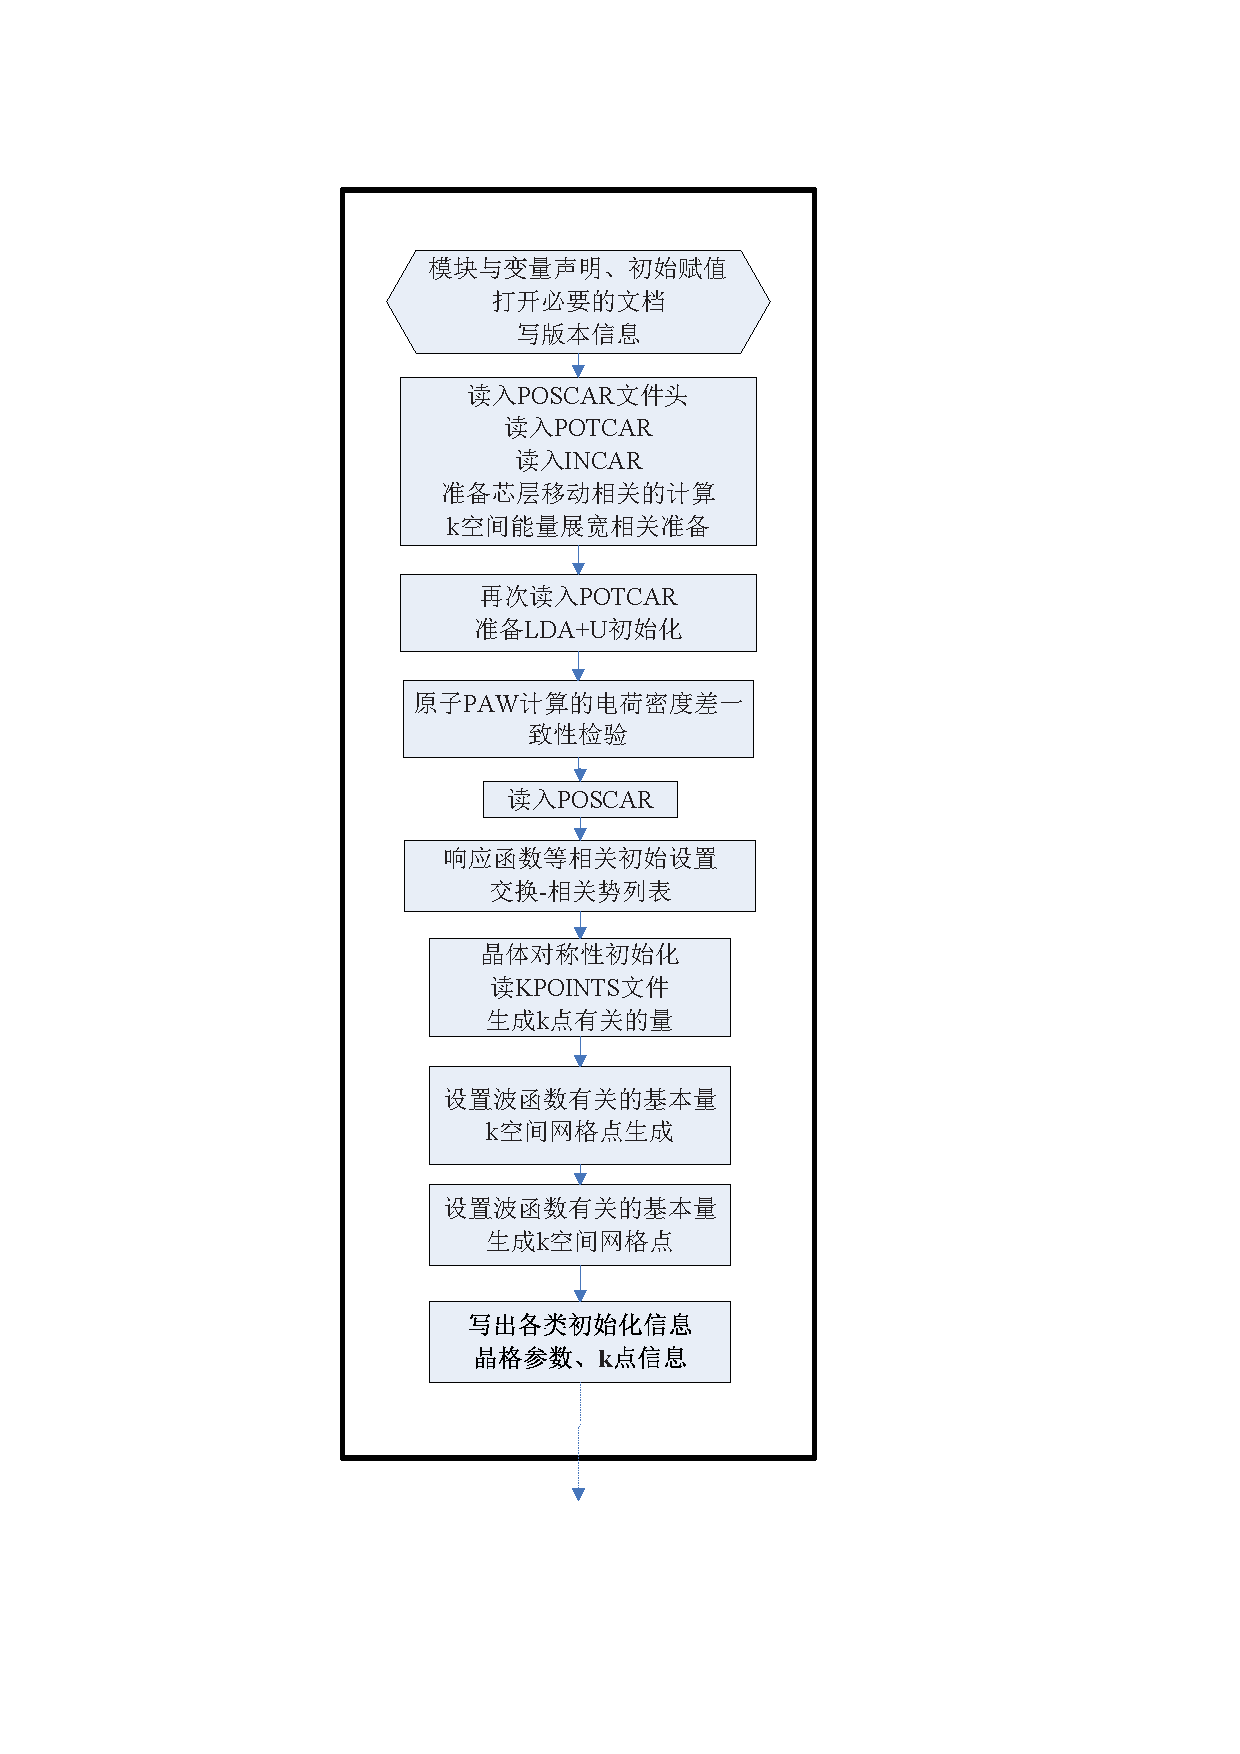
\includegraphics[height=2.65in,width=4.0in,viewport=0 360 562 720,clip]{Figures/VASP_main_Flow-1.png}
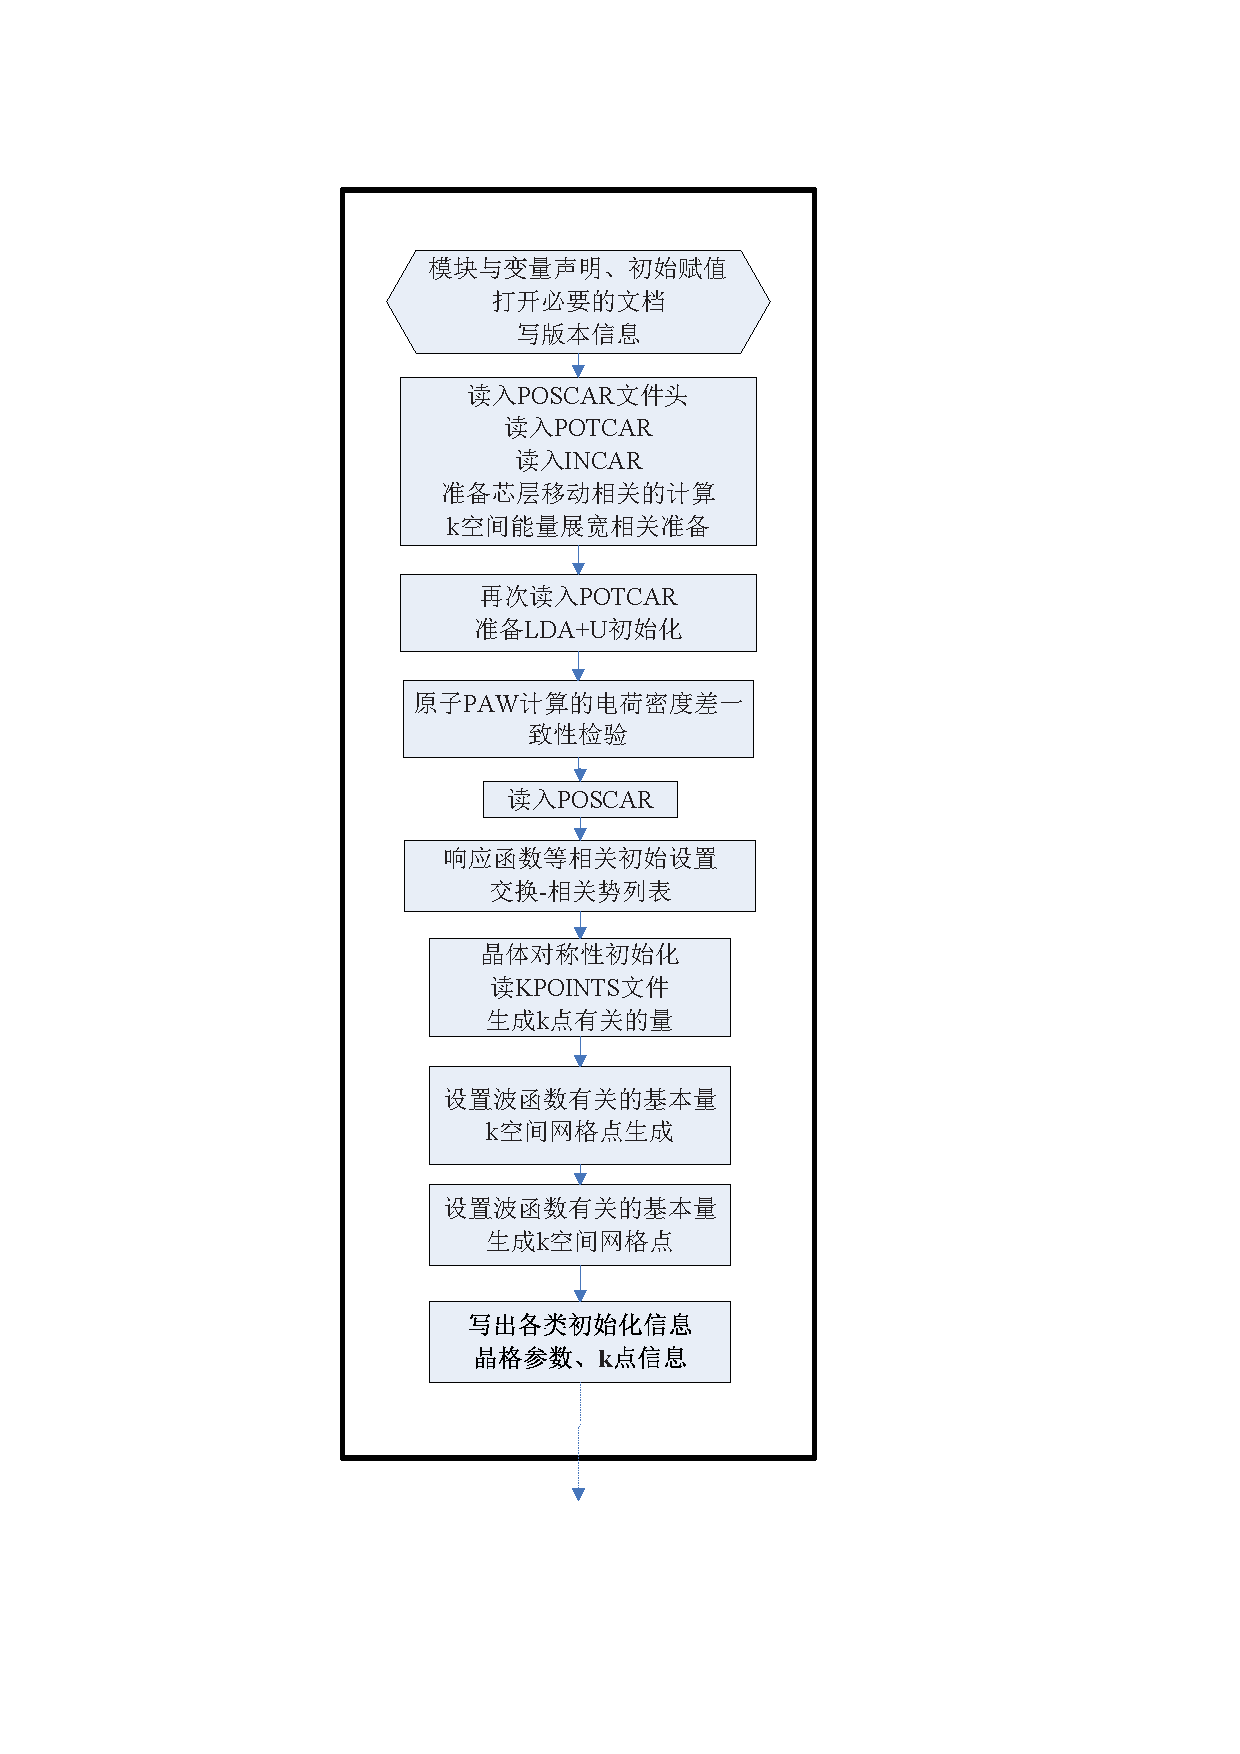
\includegraphics[height=2.65in,width=4.0in,viewport=0 0 562 360,clip]{Figures/VASP_main_Flow-1.png}
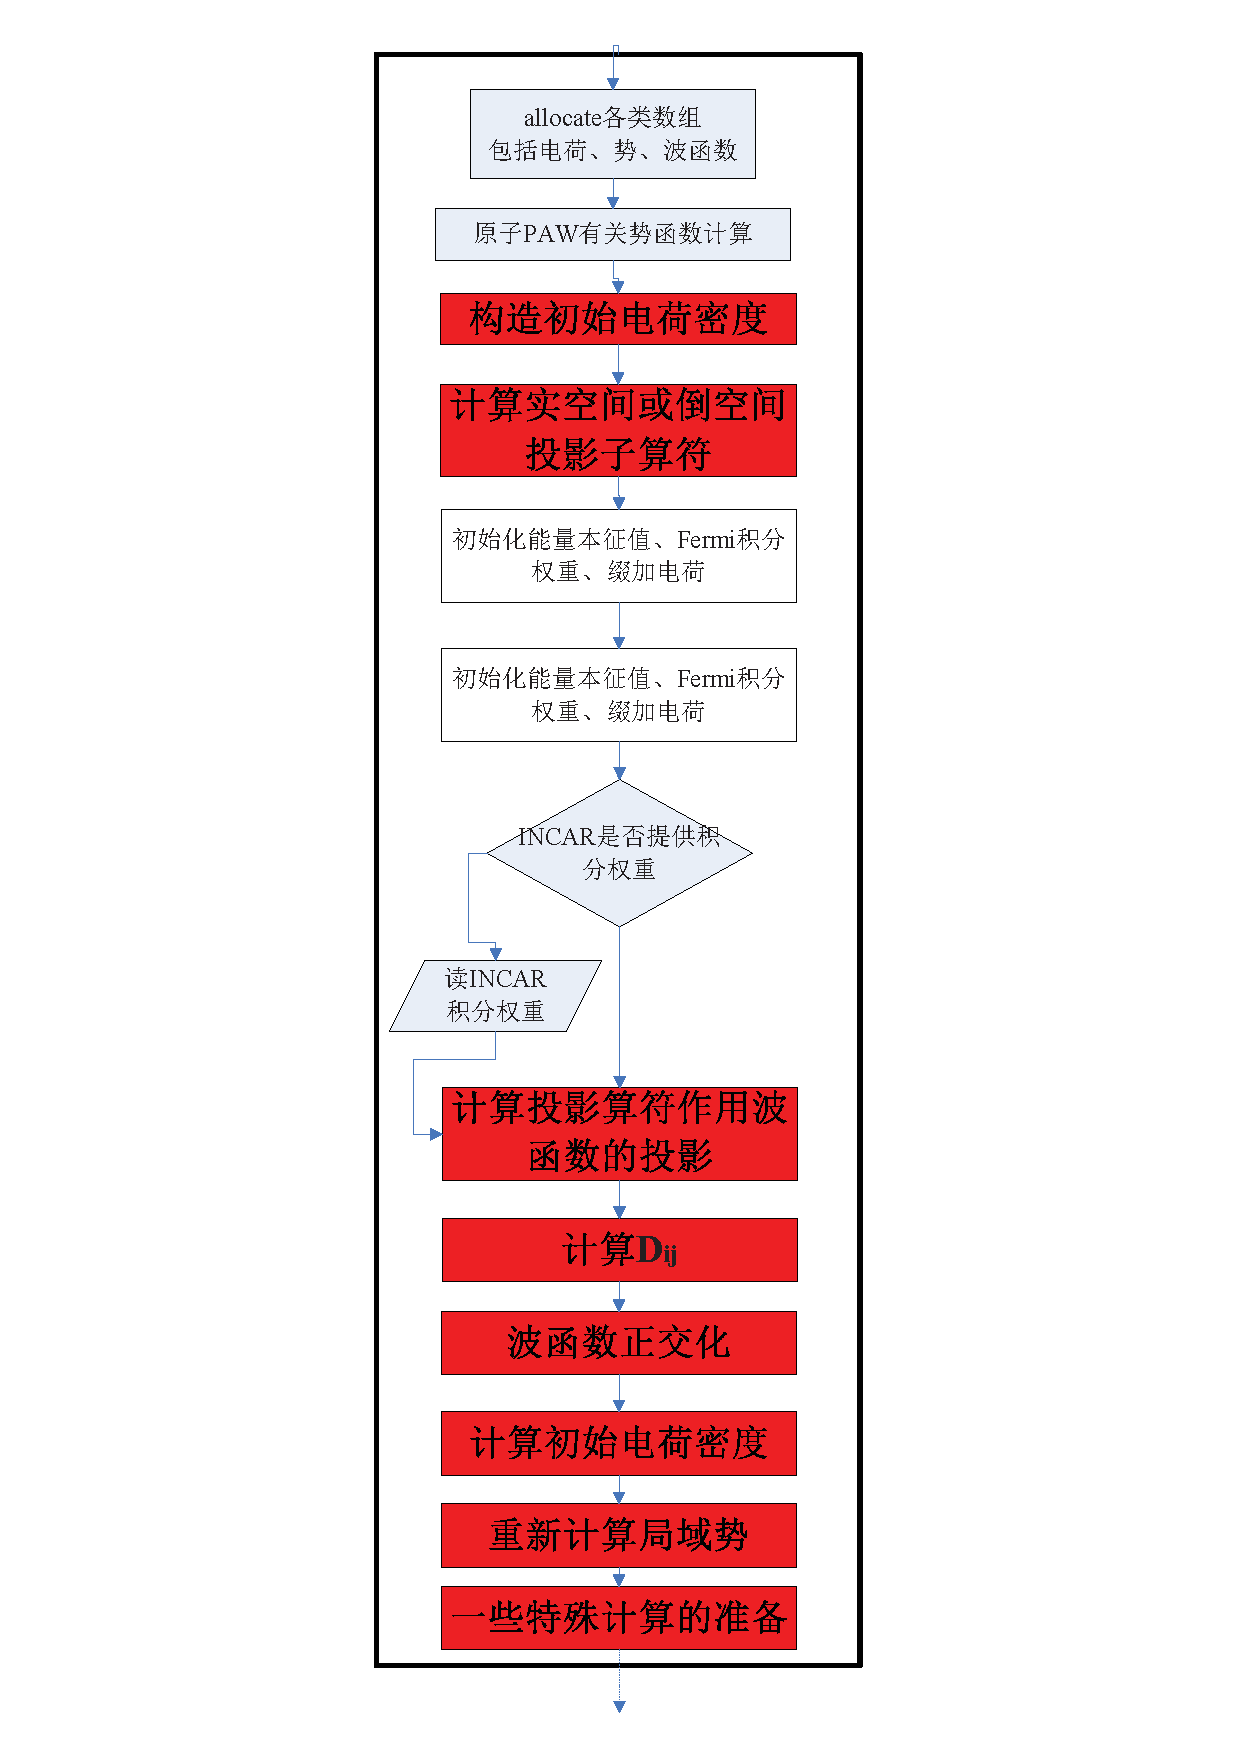
\includegraphics[height=2.35in,width=4.0in,viewport=0 370 562 680,clip]{Figures/VASP_main_Flow-2.png}
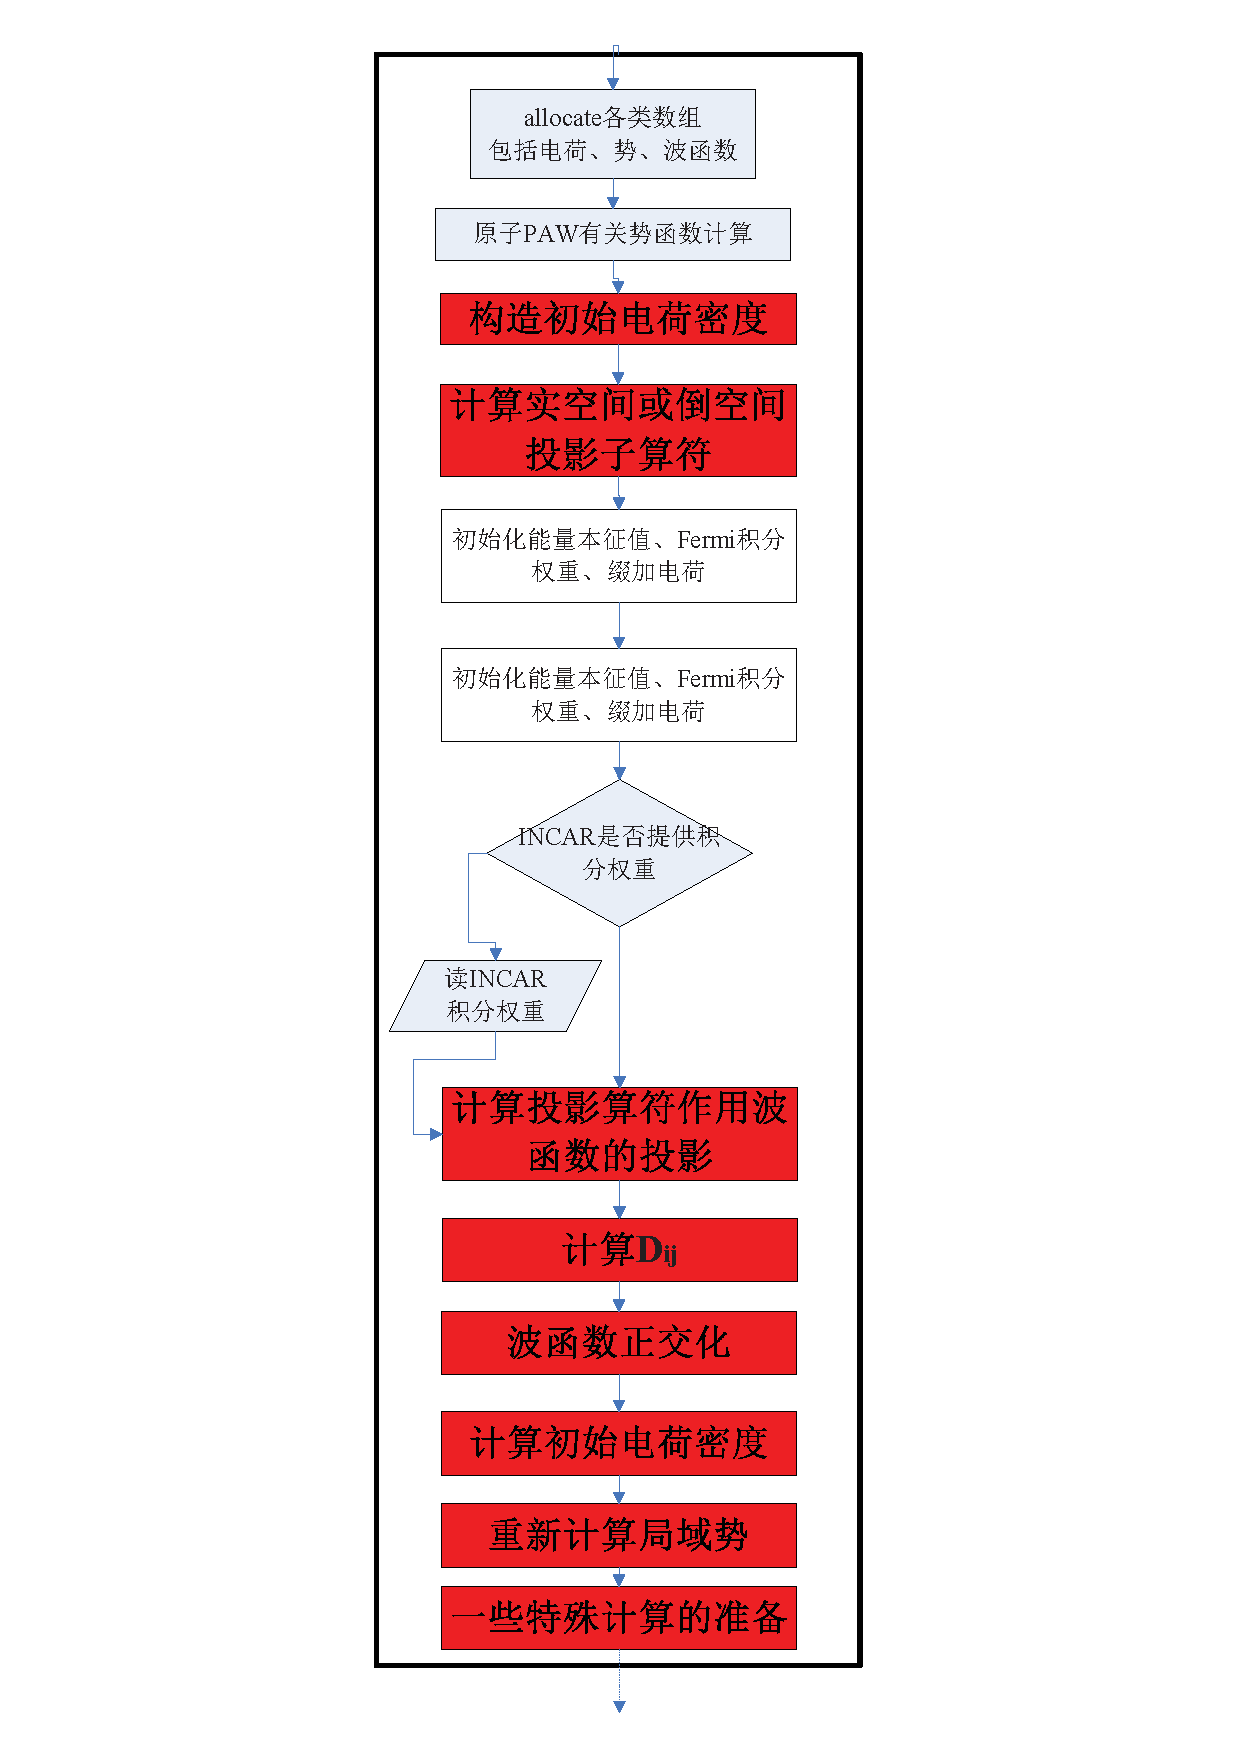
\includegraphics[height=2.50in,width=4.0in,viewport=0 0 562 370,clip]{Figures/VASP_main_Flow-2.png}
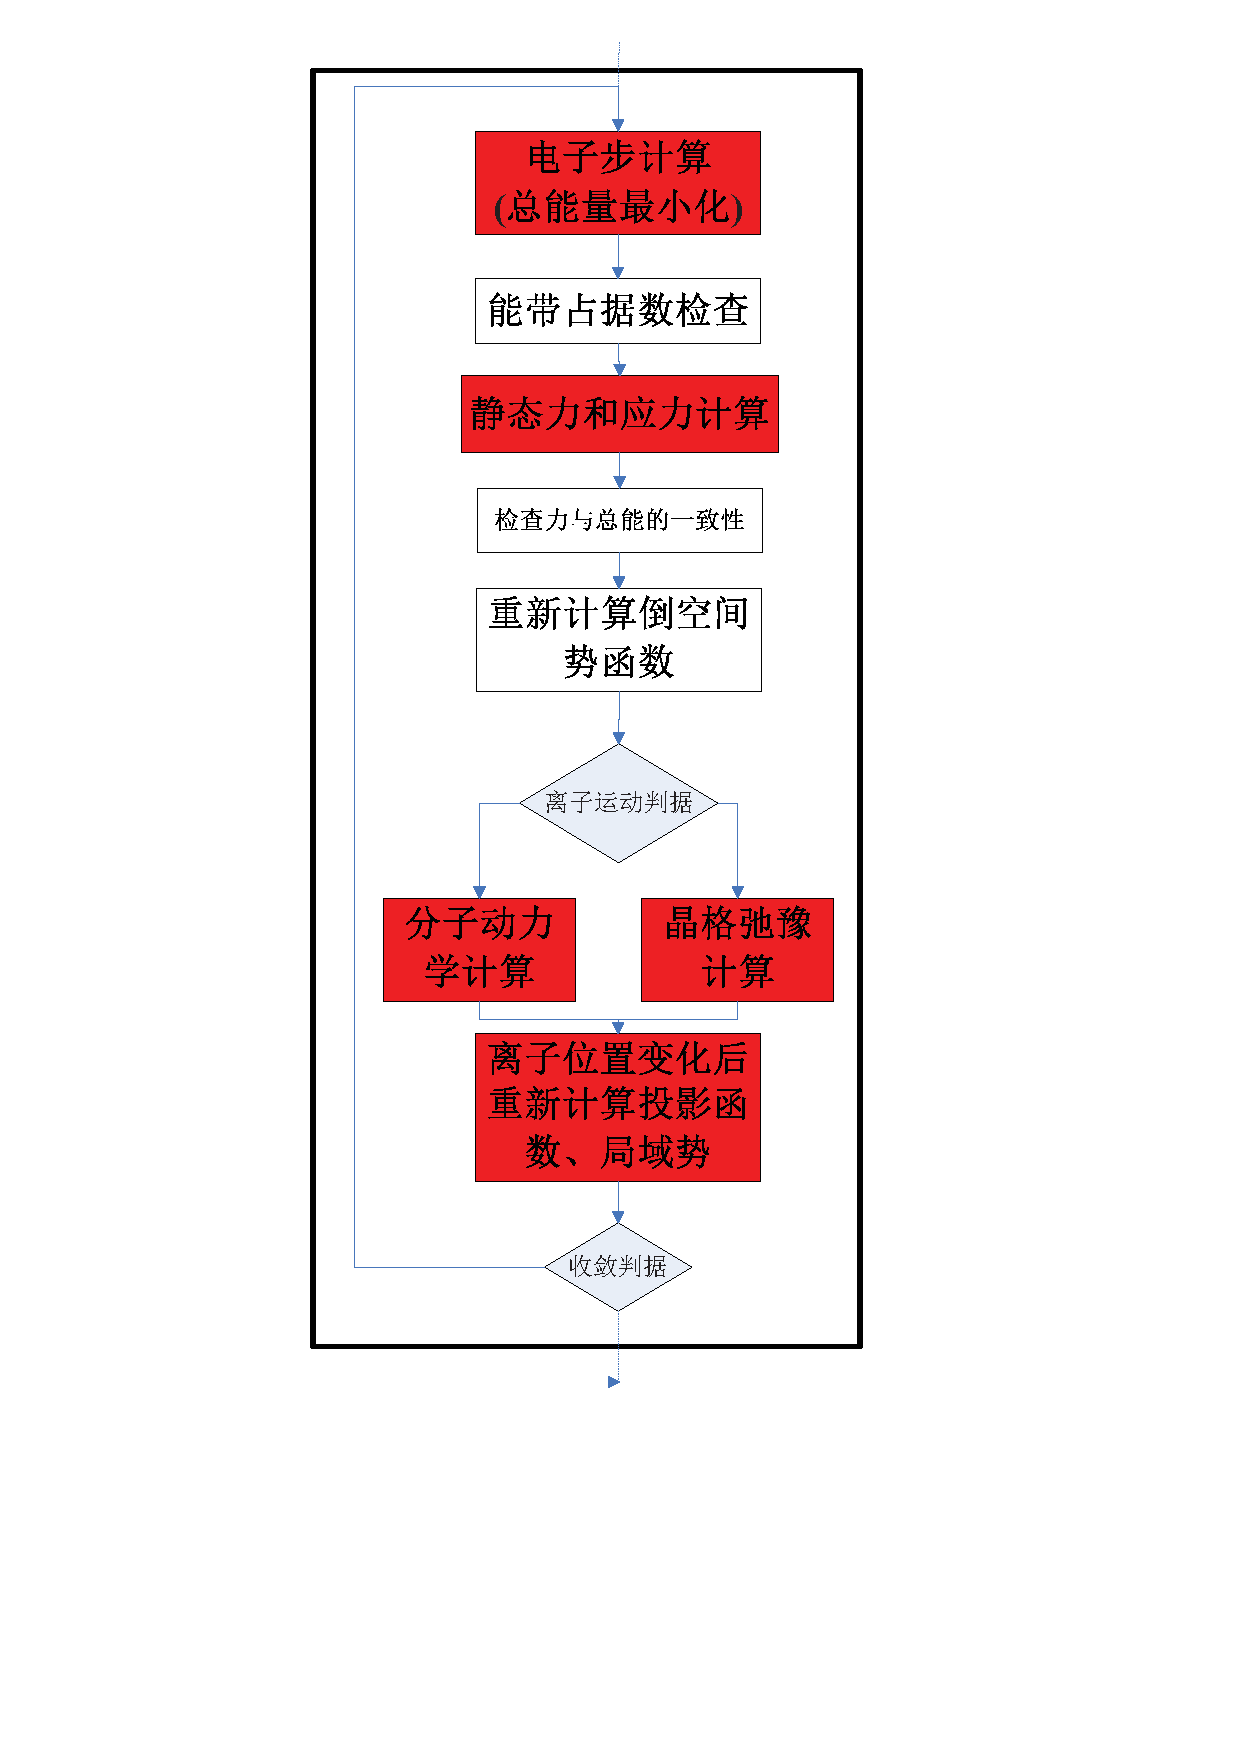
\includegraphics[height=2.45in,width=4.0in,viewport=0 350 562 660,clip]{Figures/VASP_main_Flow-3.png}
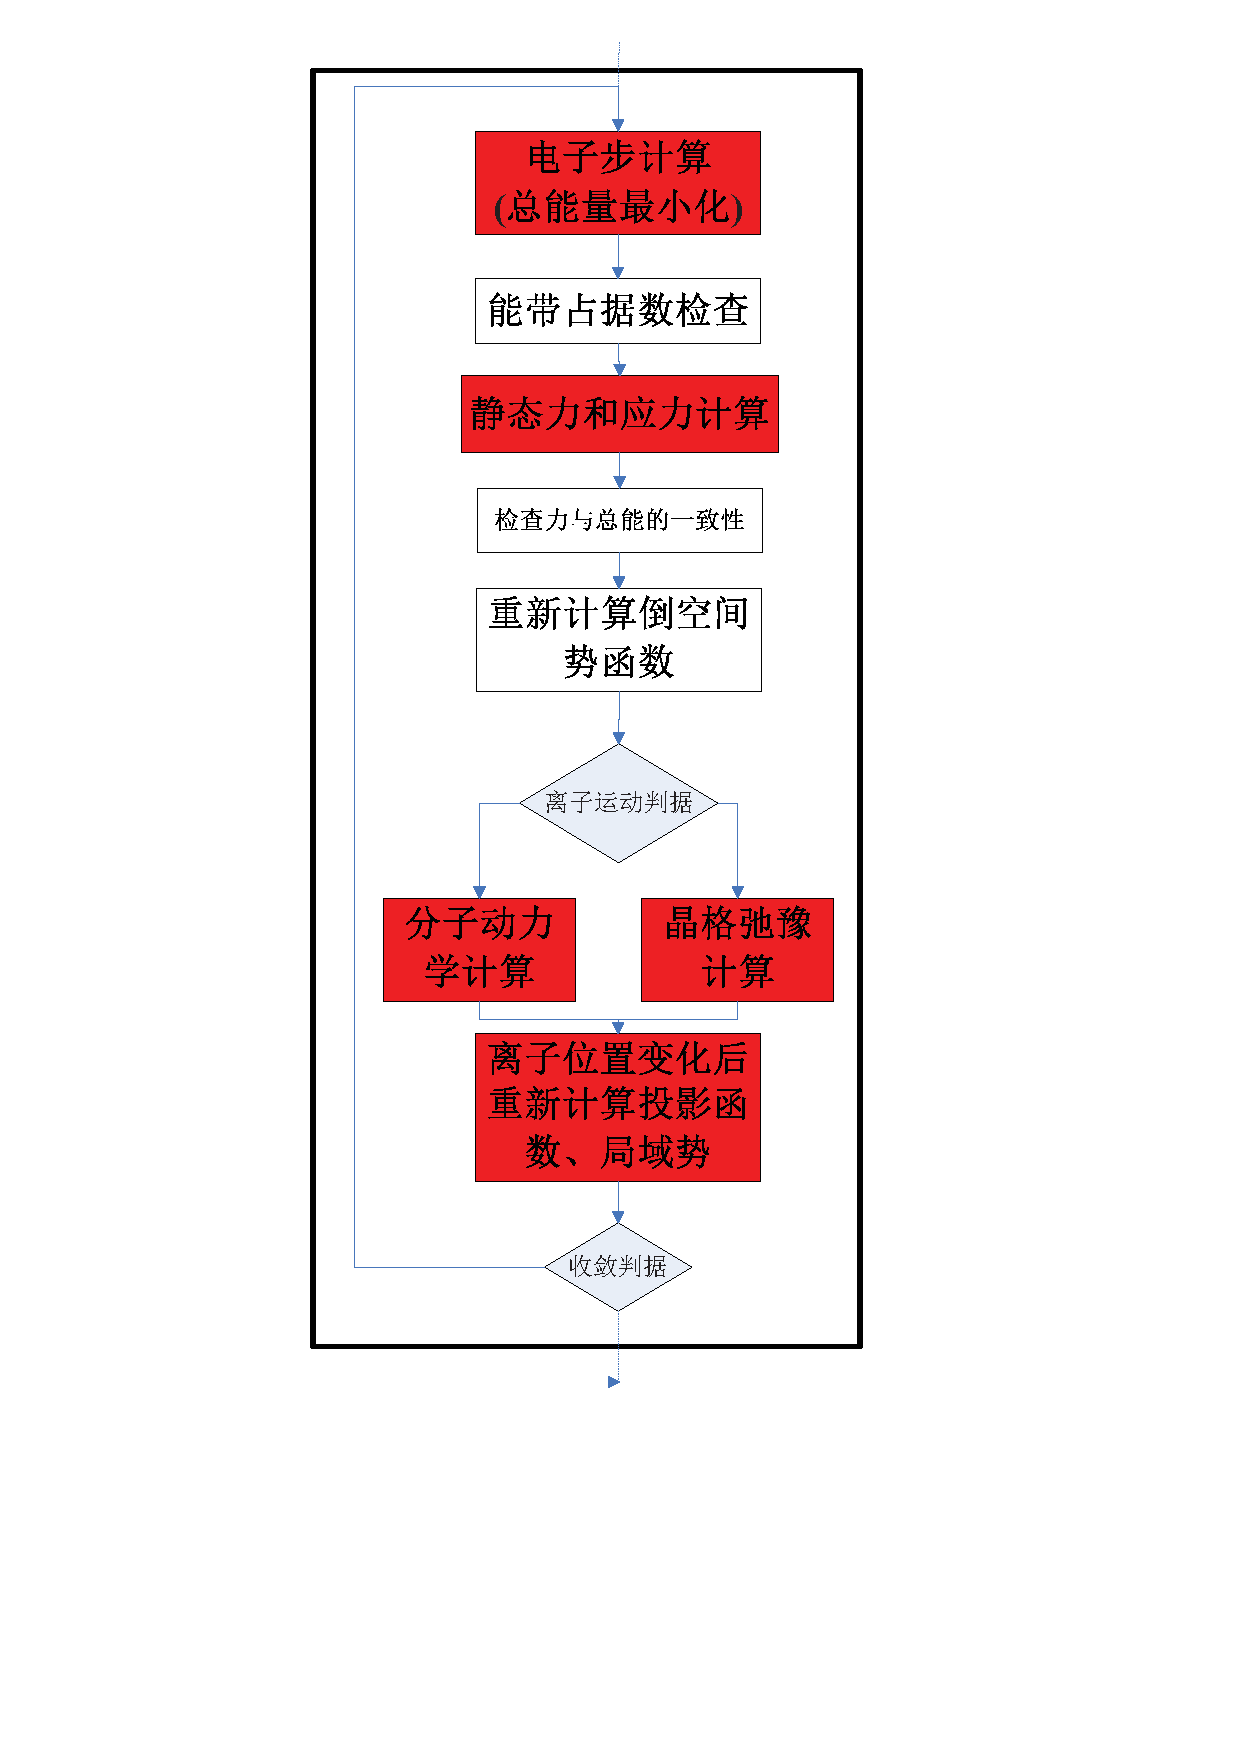
\includegraphics[height=2.50in,width=4.0in,viewport=0 0 562 350,clip]{Figures/VASP_main_Flow-3.png}
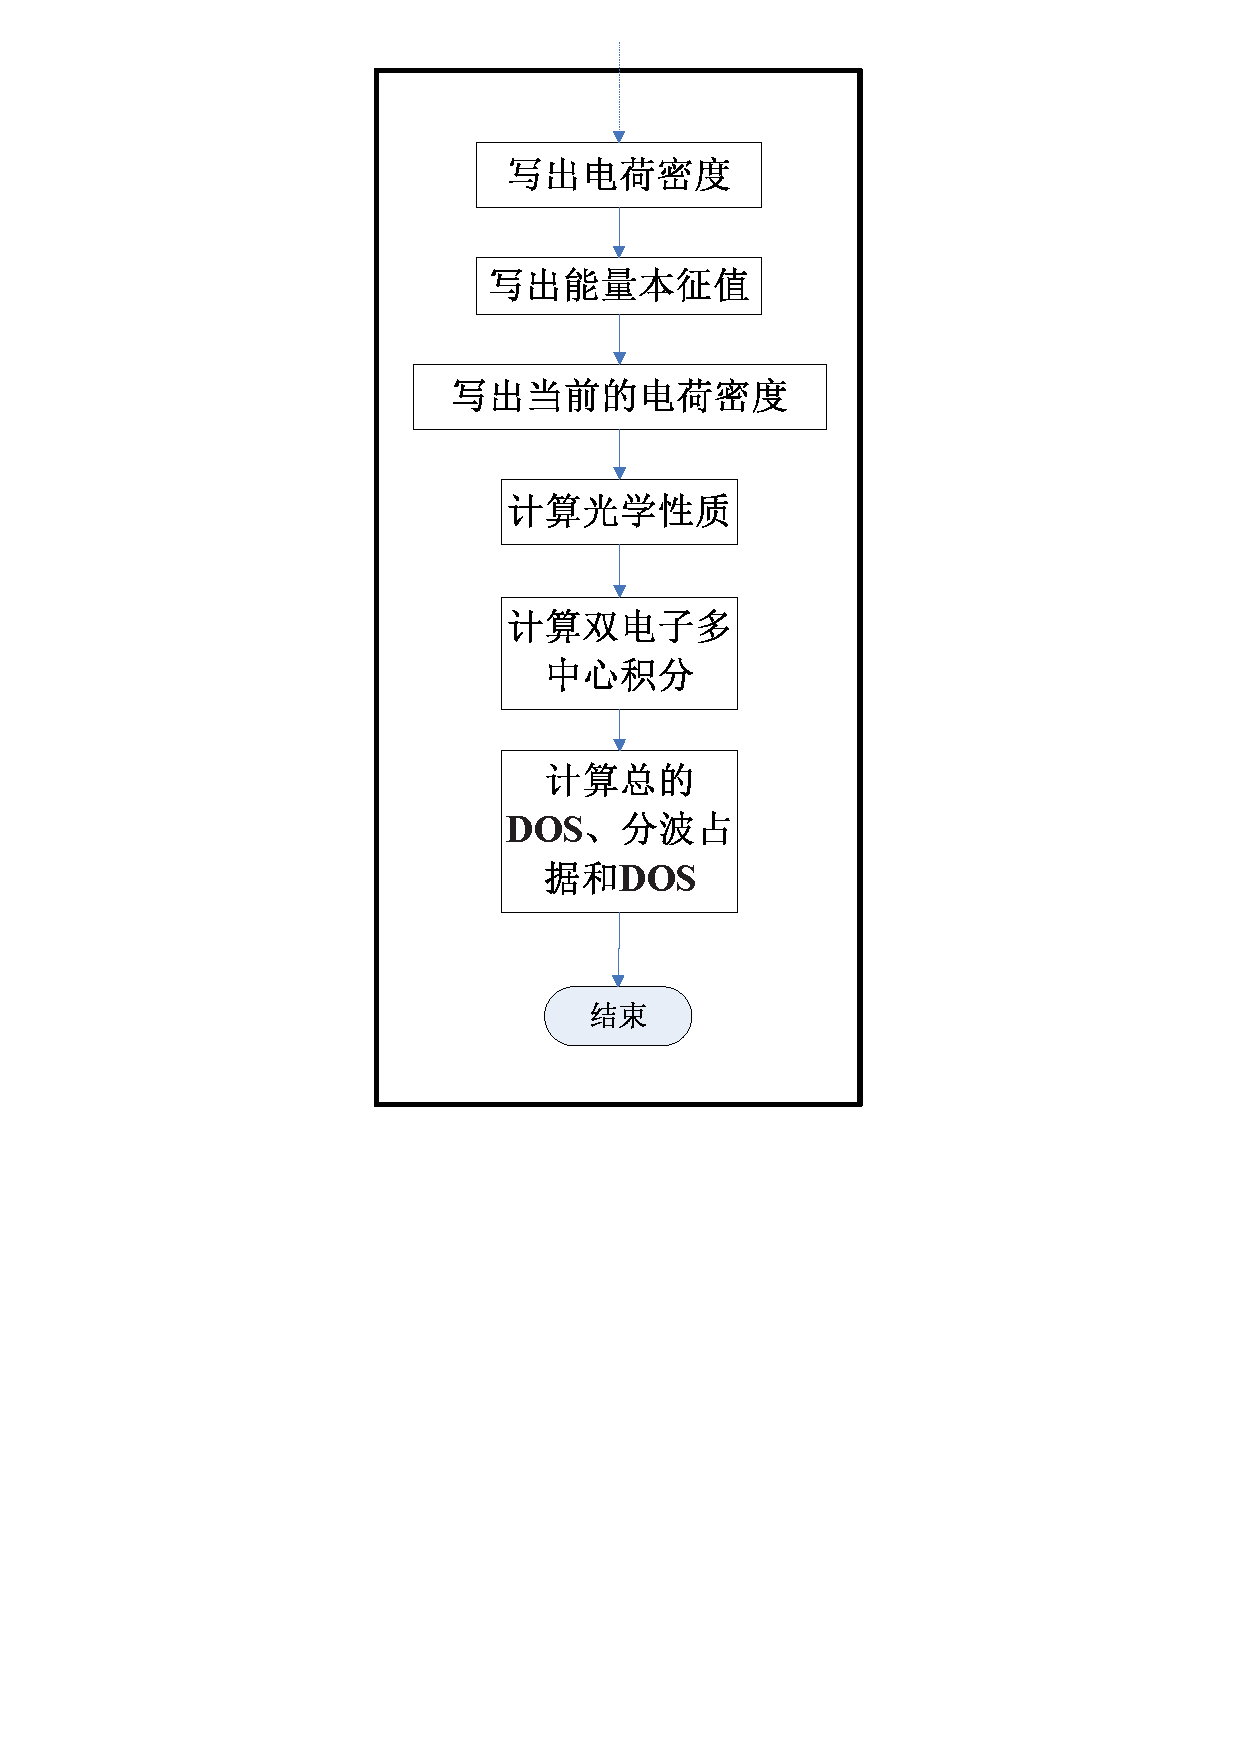
\includegraphics[height=2.30in,width=4.0in,viewport=0 215 562 530,clip]{Figures/VASP_main_Flow-4.png}
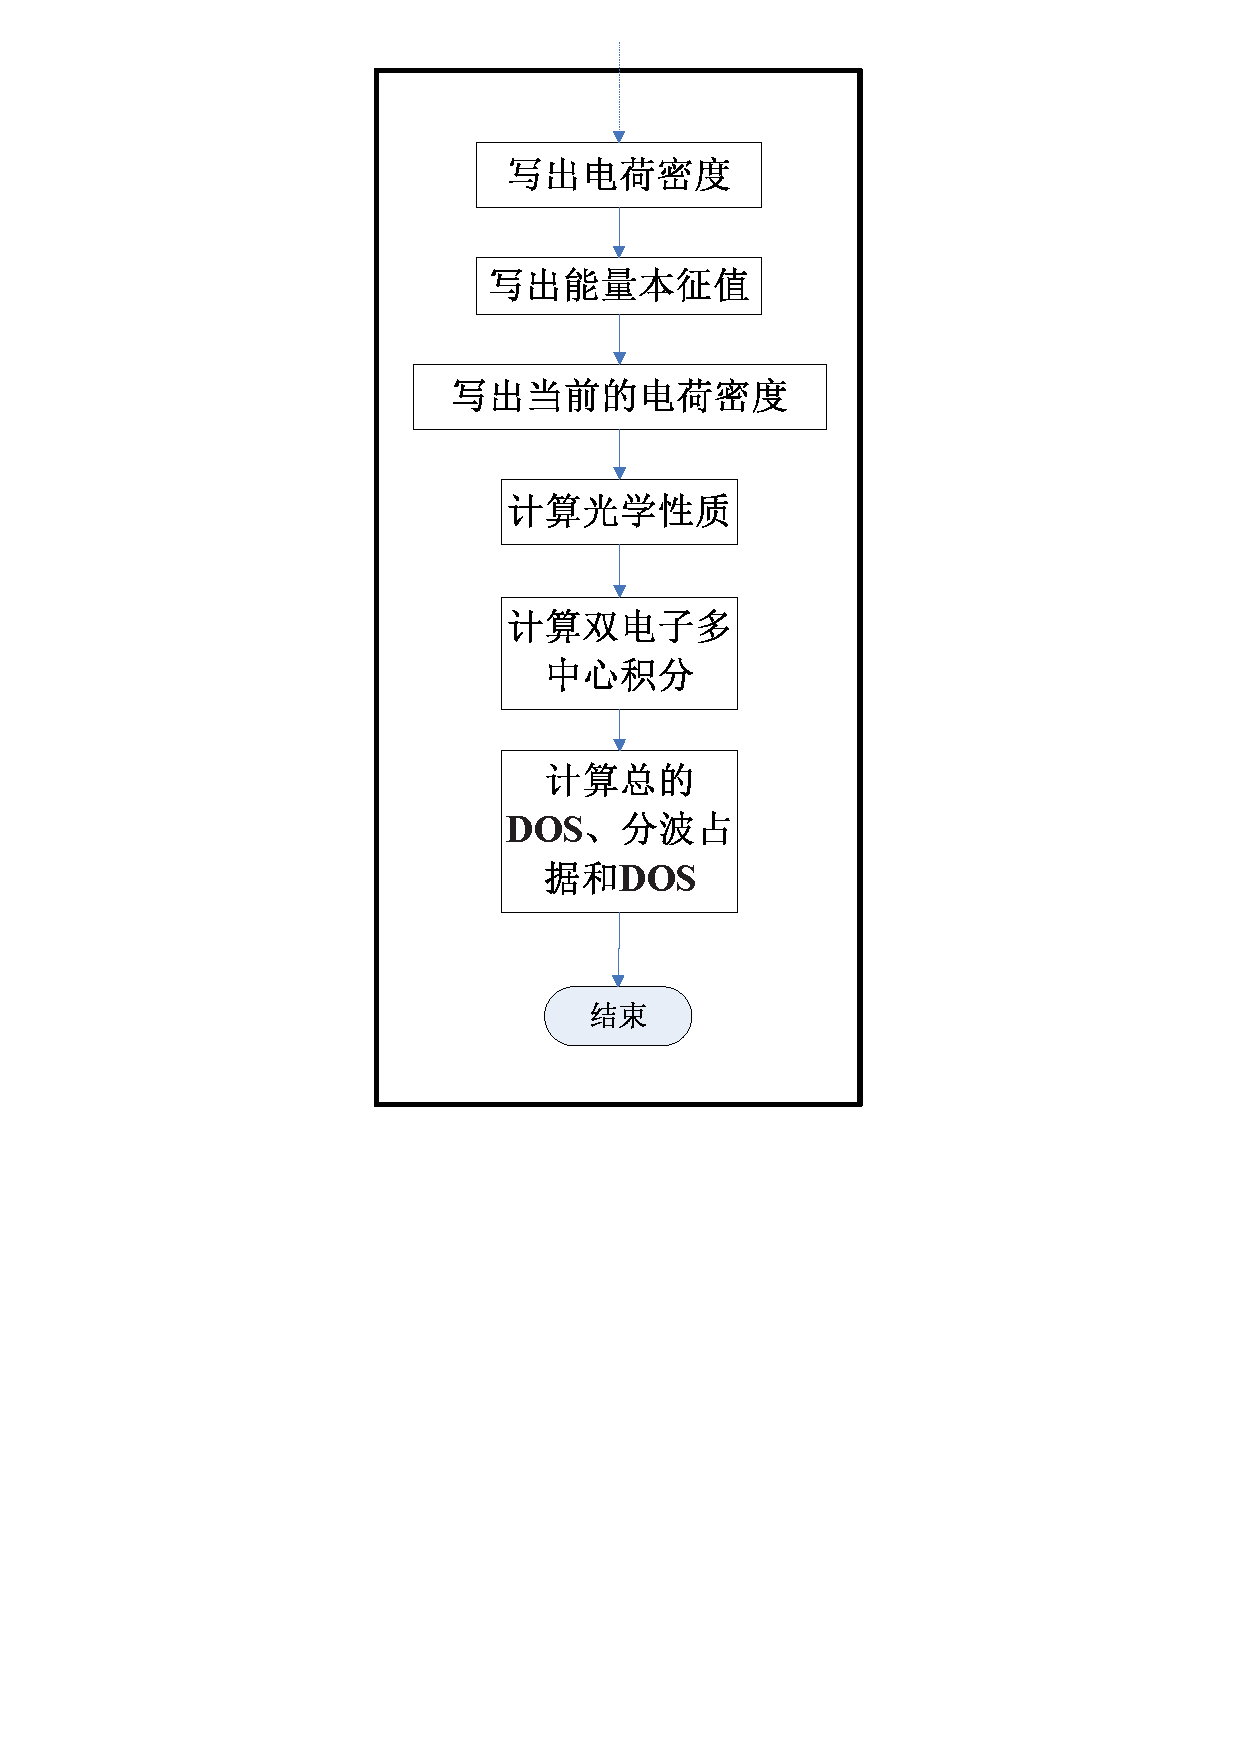
\includegraphics[height=1.40in,width=4.0in,viewport=0 0 562 215,clip]{Figures/VASP_main_Flow-4.png}
\caption{\tiny \textrm{The Flow of main program for VASP.}}%(与文献\cite{EPJB33-47_2003}图1对比)
\label{FLOW_of_VASP}
\end{figure}
\end{frame}

\section{\rm{VASP}软件的计算特色}
\frame
{
	\frametitle{双网格技术}
\begin{figure}[h!]
	\vspace{-0.15in}
\centering
%\includegraphics[height=2.7in,width=4.0in,viewport=0 0 1180 875,clip]{Figures/dual_grid.png}
\includegraphics[height=2.75in,width=4.0in,viewport=0 0 800 600,clip]{Figures/dual_grid-2.png}
\caption{\tiny \textrm{The Schematic description of the dual grid technique.}}%(与文献\cite{EPJB33-47_2003}图1对比)
\label{PAW_dualgrid}
\end{figure} 
}

\subsection{\rm{VASP}的并行}
\frame
{
	\frametitle{\textrm{VASP}的并行效率}
	与同类型软件相比,\textrm{VASP}有着优异的并行能力
\begin{figure}[h!]
	\vspace{-0.15in}
\centering
%\includegraphics[height=2.7in,width=4.0in,viewport=0 0 1180 875,clip]{Figures/dual_grid.png}
\includegraphics[height=1.55in,width=1.95in,viewport=0 0 240 200,clip]{Figures/VASP-abinit_Li128-1.png}
\includegraphics[height=1.55in,width=1.95in,viewport=0 0 240 200,clip]{Figures/VASP-abinit_Li128-2.png}
\caption{\tiny \textrm{The comparison of parallel scaling for ABINIT vs VASP.}}%(与文献\cite{EPJB33-47_2003}图1对比)
\label{ABINIT_vs_VASP}
\end{figure} 
\begin{itemize}
	\item \textrm{VASP}迭代对角化约束了矩阵的维度,减少了对角化过程中的迭代次数,保证了\textrm{MPI}并行的规模和扩展性
	\item \textrm{VASP}实施\textrm{FFT}变换时,保证各节点上处理的网格负载均衡
\end{itemize}
}

\frame
{
	\frametitle{\textrm{VASP}计算的\textrm{FFT}并行实现}
	\begin{itemize}
	     \item 中间层设计:~\textrm{FFT}网格、实空间基组与计算节点的匹配\\
		     \textcolor{red}{通过子程序\textrm{mgrid.F}生成中间层,实现并行负载与计算节点分配的匹配,减少\textrm{FFT}变换和实空间并行的节点间通信}
\begin{figure}[h!]
		\vspace{-0.25in}
	\centering
%\includegraphics[height=2.7in,width=4.0in,viewport=0 0 1180 875,clip]{Figures/dual_grid.png}
\includegraphics[height=1.0in,width=4.0in,viewport=0 0 1500 450,clip]{Figures/VASP_FFT-MPI_Reciprocal.png}
\vskip 0.5pt
\includegraphics[height=0.7in,width=4.0in,viewport=0 0 730 150,clip]{Figures/VASP_FFT-MPI_Real.png}
\caption{\tiny \textrm{VASP:~ Reciprocal-Real space layout for grids in MPI.}}%(与文献\cite{EPJB33-47_2003}图1对比)
\label{MPI-FFT}
\end{figure} 
	\end{itemize}
}

\frame
{
	\frametitle{\textrm{VASP}的通信开销}
	在高性能的计算队列中,\textrm{VASP}的并行上限可以突破256核,但当并行核数超过百核数量级,并行效率下降非常明显
\begin{figure}[h!]
	\vspace{-0.15in}
\centering
%\includegraphics[height=2.7in,width=4.0in,viewport=0 0 1180 875,clip]{Figures/dual_grid.png}
\includegraphics[height=1.55in,width=1.95in,viewport=0 0 240 200,clip]{Figures/VASP-mpi-Li128.png}
\caption{\tiny \textrm{Time spent in MPI calls with increasing the number of ranks in a VASP calculation.}}%(与文献\cite{EPJB33-47_2003}图1对比)
\label{VASP_communication}
\end{figure} 

如能对并行系统与\textrm{VASP}结合作深度改造(如国家超算天津中心方案),\textrm{VASP}的并行扩展可以到$10^4$核级别,但这一改造需要对底层代码和计算框架作较大规模改动
}

\frame
{
	\frametitle{\textrm{VASP}的\textrm{GPU}加速}
\textrm{NVIDIA}多年来致力于\textrm{VASP}的\textrm{GPU}加速,取得了一定的成效
\begin{figure}[h!]
	\vspace{-0.15in}
\centering
%\includegraphics[height=2.7in,width=4.0in,viewport=0 0 1180 875,clip]{Figures/dual_grid.png}
\includegraphics[height=1.2in,width=4.05in,viewport=0 0 850 260,clip]{Figures/VASP-GPU-CPU.png}
\caption{\tiny \textrm{Compare of VASP calculation with GPU and CPU.}}%(与文献\cite{EPJB33-47_2003}图1对比)
\label{VASP_GPU}
\end{figure} 
\begin{itemize}
	\item 通用配置下,\textrm{GPU}对\textrm{VASP}计算有加速效果,一般可提升4$\sim$6倍
	\item 矩阵对角化的并行算法限制了\textrm{GPU}在第一原理计算中的应用
	\item \textrm{GPU}加速的模式主要适合于分子动力学计算
\end{itemize}
}

%\frame[allowframebreaks]
\subsection{\rm{VASP}中的电荷密度混合与矩阵迭代对角化}
\frame
{
	\frametitle{\textrm{VASP}的优化与迭代收敛}
	\textrm{VASP}计算中,资源消耗的主要部分是求解\textrm{Kohn-Sham}方程,即偏微分方程\textrm{(Partial Differential Equations,~PDE)}的自洽迭代, 迭代过程主要包括
	\begin{itemize}
		\item 矩阵的迭代对角化
		\item 电荷密度的自洽迭代
	\end{itemize}

	\vskip 10pt
	\textrm{VASP}的计算高效得益于求解过程中中应用了多种经典优化算法,保证了迭代计算的快速收敛\upcite{CMS6-15_1996,PRB54-11169_1996}
	\begin{itemize} 
		\item 拟牛顿法\textrm{(Quasi-Newton method)}
		\item 共轭梯度法\textrm{(Conjugate Gradients method, CG)}
		\item 残差最小化\textrm{(RMM-DIIS)}方法
	\end{itemize}
}

\frame
{
	\frametitle{非线性方程的\rm{Newton~}法求根}
	\textcolor{blue}{不管哪一种数值算法,其设计原理都是将复杂转化为简单的重复,或者说,通过简单的重复生成复杂}:\\
	\textcolor{red}{在算法设计和算法实现过程中,重复就是力量}\\
迭代算法设计:~\textcolor{purple}{“速度”\textrm{vs}“稳定”}
\begin{figure}[h!]
\centering
\animategraphics[autoplay, loop, height=2.0in]{1}{Figures/OP_Newton_}{0}{17}
\label{Equation_Newon}
\end{figure}
}

\frame
{
	\frametitle{迭代优化基本思想}
	对于给定函数$f$,在极值点,函数的梯度满足
	\begin{displaymath}
		\nabla f=0
	\end{displaymath}
	可将函数极值问题转化成方程求根问题
\begin{figure}[h!]
\centering
\includegraphics[height=1.68in,width=1.95in,viewport=30 0 450 360,clip]{Figures/OP_mini-1.png}
\hskip 0.05in
\includegraphics[height=1.68in,width=1.95in,viewport=150 20 560 390,clip]{Figures/OP_mini-2.png}
\label{OP_mini}
\end{figure}
}

\frame
{
	\frametitle{最陡下降与共轭梯度}
\begin{figure}[h!]
\centering
\includegraphics[height=2.0in,width=3.5in,viewport=0 0 950 590,clip]{Figures/OP_descent_CG.png}
\label{decent_CG}
\caption{\tiny \textrm{Schematic illustration of minimization of a function in two dimensions. The steps 1,2,3,~$\cdots$ denote the steepest descent steps and - \!- \!- \!- \!- \!- the point 2$^{\ast}$ denote the conjugate gradient path that reaches the exact solution after two steps if the functional is quadratic.}}%(与文献\cite{EPJB33-47_2003}图1对比)
\end{figure}
}

\frame
{
	\frametitle{不动点问题}
	求解方程
	\begin{displaymath}
		f(\mathbf{x})=\mathbf{x}
	\end{displaymath}
	$\mathbf{x}$是函数$f(\mathbf{x})$的\textcolor{red}{不动点}\textrm{Fixed Point}
	
	对这类问题的求解,可以利用迭代关系
	\begin{displaymath}
		\mathbf{x}_{i+1}=f(\mathbf{x}_i)\qquad (i=1,2,3,\cdots)
	\end{displaymath}
	这称为\textcolor{blue}{不动点迭代法}

	{\fontsize{6.2pt}{4.2pt}\selectfont{例如求解方程
	\begin{displaymath}
%		\begin{aligned}
			\lg(10+x)~=~x%\\
			\Longrightarrow	\textcolor{blue}{x\approx 1.04309063}
%		\end{aligned}
		\end{displaymath}}}
\begin{minipage}[b]{0.35\textwidth}
		{\fontsize{3.2pt}{1.2pt}\selectfont{
	\begin{displaymath}
	\vspace{-0.11in}
		\begin{aligned}
			x_0&=1 %~\Longrightarrow 
			\\\lg(10+1)&=1.041392685\\
x_1 &=1.041392685 %~\Longrightarrow 
\\\lg(10+1.041392685)&=1.0430238558\\
x_2 &=1.043023856 %~\Longrightarrow 
\\\lg(10+1.043023856)&=1.0430880104\\
x_3 &=1.043088010 %~\Longrightarrow 
\\\lg(10+1.043088010)&=1.0443090533\\
x_4 &=1.043090533 %~\Longrightarrow 
\\\lg(10+1.043090533)&=1.04430906326\\
x_4 &=1.0430906326 %~\Longrightarrow 
\\\lg(10+1.0430906326)&=1.04430906365\\
x_5 &=1.0430906365 %~\Longrightarrow 
\\\lg(10+1.0430906365)&=1.04430906366\\
x_6 &=1.0430906366 %~\Longrightarrow 
\\\lg(10+1.0430906366)&=1.04430906366
		\end{aligned}
	\end{displaymath}}}
\end{minipage}
\hfill
\begin{minipage}[b]{0.62\textwidth}
\begin{figure}[h!]
	\vspace{-0.21in}
\centering
\includegraphics[height=1.3in,width=2.0in,viewport=0 0 2500 1600,clip]{Figures/solve_lg10.png}
%\caption{\tiny \textrm{The comparison of parallel scaling for ABINIT vs VASP.}}%(与文献\cite{EPJB33-47_2003}图1对比)
\label{solution-log_10}
\end{figure}
\end{minipage}
}

\frame
{
	\frametitle{\textrm{Residue minimization Methods}}
不动点迭代的主要问题是对初猜的依赖,很可能不收敛或线性收敛(收敛缓慢),一种求解策略是定义残量
	\begin{displaymath}
		R[\mathbf{x}]=f(\mathbf{x})-\mathbf{x}
	\end{displaymath}
	最小化残量的模$|R[\mathbf{x}]|$,特别是当残量$R[\mathbf{x}]$近似是$\mathbf{x}$的线性函数,可有\textcolor{purple}{\textrm{Jacobian}矩阵}
	\begin{displaymath}
		\mathbf{J}\equiv\dfrac{\delta R[\mathbf{x}]}{\delta\mathbf{x}}
	\end{displaymath}
	然后可以用\textrm{Quasi-Newton}方法最小化残量\\具体地可通过迭代关系求解原方程的解
	\begin{displaymath}
		\mathbf{x}_{i+1}=\mathbf{x}_{i}-\mathbf{J}^{-1}R[\mathbf{x}_{i}]
	\end{displaymath}
		但是一般来说\textrm{Jacobian}矩阵很可能未知(或者很难求逆),只有另图别策(在\textrm{Krylov}子空间中迭代求解),一般常用的方法有
		\begin{itemize}
			\item 迭代子空间求逆(\textrm{Discret Inversion in the Iterative Subspace,~DIIS})
			\item \textrm{Anderson}加速或\textrm{Anderson}混合
		\end{itemize}
}
	
\frame[allowframebreaks]
{
	\frametitle{电荷密度混合收敛算法}
	根据\textrm{DFT},搜索基态电荷密度的过程就是能量泛函优化的过程,可以通过此前讨论的迭代算法实现:\\
%由初猜电荷密度出发,
	\begin{displaymath}
		R[\rho_{\mathrm{in}}]=\rho_{\mathrm{out}}[\rho_{\mathrm{in}}]-\rho_{\mathrm{in}}
	\end{displaymath}
	自洽迭代收敛时,残矢模量$\langle R[\rho_{\mathrm{in}}]|R[\rho_{\mathrm{in}}]\rangle~\rightarrow~0$

	\begin{itemize}
		\item 线性混合:\\
			如果电荷密度自洽迭代的每一步只保留当前步的电荷密度信息,就是线性电荷密度的线性混合
			\begin{displaymath}
				\rho_{\mathrm{in}}^{m+1}=\rho_{\mathrm{in}}^{m}+\gamma R[\rho_{\mathrm{in}}^m]
			\end{displaymath}
	显然,这种线性混合收敛比较慢,应用\textrm{Jacobian}矩阵相关的知识,通过选择\textrm{Preconditioning~}函数,加速自洽迭代的收敛
	\begin{displaymath}
		\rho_{\mathrm{in}}^{m+1}=\rho_{\mathrm{in}}^{m}+\mathbf{G}^1R[\rho_{\mathrm{in}}^m]
	\end{displaymath}
		\item \textrm{Kerker~}混合:\\%~
			以平面波为基,选择的\textrm{Preconditioning~}函数为
			\begin{displaymath}
				G_q^1=A\dfrac{q^2}{q^2+q_0^2}\quad\mbox{一般取$A=0.8$,$q_0$则可根据体系优化}
			\end{displaymath}
		\item \textrm{Pulay}混合:\\
			优化过程中,保留此前若干步的输入电荷密度和残矢,用于迭代的优化电荷密度由此前的电荷密度线性组合得到
			\begin{displaymath}
				\rho_{\mathrm{in}}^{\mathrm{opt}}=\sum_i\alpha_i\rho_{\mathrm{in}}^i
			\end{displaymath}
			\textcolor{magenta}{假设残矢与密度有相同的线性化形式}
			\begin{displaymath}
				R[\rho_{\mathrm{in}}^{\mathrm{opt}}]=R\bigg[\sum_i\alpha_i\rho_{\mathrm{in}}^i\bigg]=\sum_i\alpha_iR[\rho_{\mathrm{in}}^i]
			\end{displaymath}
			在归一化约束条件$\sum\limits_{i}\alpha_i=1$下,通过最小化残矢模量$\langle R\big[\rho_{\mathrm{in}}^{\mathrm{opt}}\big]|R\big[\rho_{\mathrm{in}}^{\mathrm{opt}}\big]\rangle$,得到优化电荷密度,可以得到优化系数$\alpha_i$
	\begin{displaymath}
		a_i=\dfrac{\sum\limits_{j}A_{j,i}^{-1}}{\sum\limits_{j,k}A_{j,k}^{-1}}\qquad A_{j,k}=\langle R[\rho_{\mathrm{in}}^{j}]|R[\rho_{\mathrm{in}}^{k}]\rangle 
	\end{displaymath}
\item \textrm{Brondey}混合:\\
	这是所有自洽求解\textrm{Kohn-Sham}方程方法中最复杂的,属于准-\textrm{Newton}类方法。在迭代过程中,用近似方法不断对\textrm{Jacobian~}矩阵(或逆矩阵)逼近\\
	每次自洽迭代中并不需要保存全部$N\times N$的\textrm{Jacobian}矩阵,只需要存储$N$-维矢量\\
	\textcolor{purple}{残矢可以线性化地表示为}
	\begin{displaymath}
		R[\rho]=R[\rho_{\mathrm{in}}^m]-\mathrm{J}^m(\rho-\rho_{\mathrm{in}}^m)
	\end{displaymath}
	这里$\mathbf{J}^m$是对\textrm{Jacobian~}矩阵的近似($(\mathbf{J}^m)^{-1}$是\textrm{Jacobian}矩阵的逆阵,习惯上取$\mathbf{G}^m=(\mathbf{J}^m)^{-1}$),由此可有迭代电荷密度
	\begin{displaymath}
		\rho_{\mathrm{in}}^{m+1}=\rho_{\mathrm{in}}^m+(\mathbf{J}^m)^{-1}R[\rho_{\mathrm{in}}^m]
	\end{displaymath}
	此类方法因为迭代中$\mathbf{J}^m$的变化形式不同,可以选择多种方案\\
	定义误差函数
	\begin{displaymath}
		E=w_0||\mathbf{G}^{m+1}-\mathbf{G}^m||^2+\sum_{i=1}^mw_i||\Delta\rho^i+\mathbf{G}^{m+1}\Delta R^i||^2
	\end{displaymath}
	这里$||A||^2=\langle A|A\rangle$,$w_i$是权重因子,并且有
	\begin{displaymath}
		\begin{aligned}
			\Delta\rho^i=&\rho_{\mathrm{in}}^{i+1}-\rho_{\mathrm{in}}^{i}\\
			\Delta R[\rho^i]=&R[\rho_{\mathrm{in}}^{i+1}]-R[\rho_{\mathrm{in}}^{i}]
		\end{aligned}
	\end{displaymath}
	\begin{itemize}
		\item 误差函数的第一项要求\textrm{Jacobian}矩阵的逆阵在迭代中变化不大,并有$w_0\rightarrow0$
		\item 误差函数的第二项要求模$||\Delta\rho^i+\mathbf{G}^{m+1}\Delta R^i||$足够小
	\end{itemize}
	用最小二乘法确定最小化误差,可以确定$\mathbf{G}^m$
	\begin{displaymath}
		\mathbf{G}^{m+1}=\mathrm{G}^1-\sum_{k=1}^m|\mathbf{Z}_k^m\rangle\langle\Delta R^k|
	\end{displaymath}
	其中
	\begin{displaymath}
		\begin{aligned}
			|\mathbf{Z}_k^m\rangle=&\sum_{n=1}^m\beta_{kn}w_kw_n|u^n\rangle+\sum_{n=1}^{m-1}\bar{\beta}_{kn}|\mathbf{Z}_n^{m-1}\rangle\\
			|u^n\rangle=&\mathbf{G}^1|\Delta R^n\rangle+|\Delta \rho^n\rangle
		\end{aligned}
	\end{displaymath}
	而$\beta_{kn}$和$\bar\beta_{kn}$由下式给出
	\begin{displaymath}
		\begin{aligned}
			\beta_{kn}=&\big(w_0^2+\bar A\big)_{kn}^{-1},\qquad \bar A_{kn}=w_kw_n\langle\Delta R^n|\Delta R^k\rangle\\
			\bar\beta_{kn}=&\delta_{kn}-\sum_{j=1}^mw_kw_j\beta_{kj}\langle\Delta R^n|\Delta R^j\rangle
		\end{aligned}
	\end{displaymath}
		{\fontsize{7.2pt}{4.2pt}\selectfont{
	不难看出\\$w_0\rightarrow 0$并且$w_0\ll w_n$,该方法就得到\textrm{Pulay}方法\\
	而一旦$w_0\rightarrow 0$时,$w_n$的选择,完全不会影响$\mathbf{G}^{m+1}$,因此取$w_n=1$可有
	\begin{displaymath}
		\mathbf{G}^m=\mathbf{G}^1-\sum_{k,n=1}^{m-1}\beta_{kn}|u^n\rangle\langle\Delta R^k|
	\end{displaymath}
而如果令$w_i=0$并要求$w_0\ll w_m$,有
\begin{displaymath}
	\begin{aligned}
		|\mathbf{Z}_k^m\rangle=&|\mathbf{Z}_k^{m-1}\rangle\qquad k<m\\
		|\mathbf{Z}_m^m\rangle=&\dfrac1{||\Delta R^m||^2}\bigg(|u^m\rangle-\sum_{k=1}^{m-1}\langle\Delta R^k|\Delta R^m\rangle|\mathbf{Z}_k^{m-1}\rangle\bigg)
	\end{aligned}
\end{displaymath}
}}
	\end{itemize}
}

\frame
{
	\frametitle{矩阵的迭代对角化}
	\begin{itemize}
		\item 矩阵的直接对角化计算复杂复 $O(N^3)$
		\item 矩阵的迭代对角化计算复杂度 $O(N_0^2\times N\ln N)\quad N_0\ll N$
	\end{itemize}
	\textcolor{blue}{迭代求本征值的思想是\textrm{Jacobian~}于\textrm{1846~}年提出的}\upcite{Crelle30-51_1846}\\
	其基本思想是
	\begin{displaymath}
		(H-\varepsilon^n)|\psi^n\rangle=|R[\psi^n]\rangle
	\end{displaymath}
	这里$n$是迭代步数,$|\psi^n\rangle$和$\varepsilon^n$分别是本征态和本征值,$|R[\psi^n]\rangle$是残差矢量
	\vskip 10pt
	{\fontsize{7.2pt}{1.2pt}\selectfont{
	在电子态计算过程中,选择适当的基函数,可以使\textrm{Schr\"odinger~}方程的矩阵接近对角阵\\因此可有
	\begin{displaymath}
		\begin{aligned}
			|\psi^{n+1}\rangle=&\mathbf{D}^{-1}(\mathbf{H}-\varepsilon)|\psi^n\rangle+|\psi^n\rangle=\delta|\psi^{n+1}\rangle+|\psi^n\rangle\\
		\mathbf{D}\delta\psi^{n+1}=&R[\psi^n]
		\end{aligned}
	\end{displaymath}
	这里$\mathbf{D}$是非奇异矩阵,与$\mathbf{H}$矩阵有关,也叫''预处理矩阵'',可根据需要选取多种形式
	\begin{itemize}
		\item 要求$\mathbf{D}$比原始的$\mathbf{H}-\varepsilon$更易求逆阵
		\item 要求$\mathbf{D}$使得修正项$\delta\psi^{n+1}$能够使$\psi^n$尽可能接近正确的本征矢
	\end{itemize}
}}
}

\frame
{
	\frametitle{矩阵的迭代对角化}
	``预处理矩阵''%$\mathbf{K}$
	的作用,是使\textcolor{red}{函数(泛函)对变量的依赖趋于“同质”(\textrm{isotropic})},即函数曲线与不同变量的依赖关系趋同

	具体到电子结构求解:~
	\begin{itemize}
		\item \textcolor{blue}{平面波基}\\
			基函数$\mathrm{e}^{\mathrm{i}\vec G_m\cdot\vec r}$对波函数$\psi_{\vec k_i+\vec G}^n(\vec r)$的贡献为$c_{i,m}^n(\vec k)$\\
		{\fontsize{7.2pt}{4.2pt}\selectfont{
		在能量泛函表达式中,高频(大的$\vec G_m$)部分比低频(小的$\vec G_m$)贡献大得多}}\\
			\textrm{preconditioning}\textcolor{blue}{要使不同频率对能量泛函贡献趋同}:\\
			\textcolor{red}{不同本征矢的修正项趋同,而与相应的能量本征值无关。}取
	\begin{displaymath}
		K(x)=\dfrac{27+18x+12x^2+8x^3}{27+18x+12x^2+8x^3+16x^4}
	\end{displaymath}
	此处定义
	\begin{displaymath}
		x_i^n(\vec G_m)=\dfrac12\dfrac{|\vec k+\vec G_m|^2}{E^{\mathrm{kin}}(\mathbf{R}^n)}
	\end{displaymath}
	\textcolor{purple}{$x_i^n(\vec G_m)$表示对$n$次迭代后本征态$i$中平面波组分$|\vec k_i+\vec G_m|$动能贡献的调整比例}
	\end{itemize}
}

\frame
{
	\frametitle{矩阵迭代对角化}
	稀疏矩阵求解的\textrm{Lanczos}优化过程\upcite{Elect_Stru,Comp_Phys},只变动一个分量$\mathbf{c}_I$的前提下
	\begin{displaymath}
		\dfrac{\partial\rho}{\partial\mathbf{c}_I}\bigg|_{\mathbf{c}_I+\delta_I}=0
	\end{displaymath}
	是可以精确求解的,其解为
	\begin{displaymath}
		\delta_I=(\rho(\mathbf{c}_0)-\mathbf{H}_{II})^{-1}\mathbf{q}_I\qquad\mbox{这里}\mathbf{q}=(\mathbf{H}-\rho\mathbf{I})\mathbf{c}_0
	\end{displaymath}
	不难看出,矢量$\mathbf{q}$就对应\textrm{Jacobi}迭代中用于判断收敛的残差矢量

更一般地,求解方程
	\begin{displaymath}
		\dfrac{\partial\rho}{\partial\mathbf{c}}\bigg|_{\mathbf{c}+\mathbf{\delta}}=0
	\end{displaymath}
	将方程展开到二阶近似,不难有
	\begin{displaymath}
		(\rho-\mathbf{H}_{II})\delta_I\approx \mathbf{q}_I+\sum_{J\neq I}\delta_J+(\rho-\lambda)\mathbf{c}_I
	\end{displaymath}
	实际计算中选则$\delta_I=(\rho(\mathbf{c}_0)-\mathbf{H}_{II})^{-1}\mathbf{q}_I$并不是方程的解的好的近似,\textcolor{purple}{好处是计算比较简单}
}

\frame
{
	\frametitle{\textrm{Block-Davison algorithm}}
	\textrm{Davidson}方法是求解大型稀疏矩阵的少量本征值问题提出来的,结合了\textrm{Lanczos}优化和\textrm{Jacobi}迭代的优点,简言之就是改进初猜,不用$\mathbf{H}\mathbf{c}_0$,而改用计算简单的$\delta_I=(\rho(\mathbf{c}_0)-\mathbf{H}_{II})^{-1}\mathbf{q}_I$形式
	\vskip 10pt
	应用\textrm{Davison}方法可以快速地依次求解稀疏矩阵的少量本征值和本征矢,将该方法推广为同时求解若干个本征态,即块-\textrm{Davidson}方法
	{\fontsize{6.2pt}{1.2pt}\selectfont{
		\begin{itemize}
			\item 选取合适数目正交归一的向量$\mathbf{c}_1,\mathbf{c}_2,\cdots, \mathbf{c}_n$作为初猜子空间的基组, 计算并储存向量$\mathbf{H}\mathbf{c}_i$和矩阵元$\mathbf{H}=\langle\mathbf{c}_i|\mathbf{H}|\mathbf{c}_j\rangle$ 
			\item 对角化矩阵,得到本征值$\lambda^{n}$和本征矢$\mathbf{a}^{n}$
			\item 构造残量矢量$\mathbf{q}_M=(\mathbf{H}-\lambda^{(M)}\mathbf{I})\mathbf{a}^{(M)}~\mbox{其中}\mathbf{a}^{(M)}=\sum\limits_{i=1}^M a_i^{(M)}\mathbf{a}_i$
			\item 根据模长$||\mathbf{q}_M||$判断迭代收敛情况
			\item 构造$\delta_{I,M+1}=(\lambda^{(M)}-\mathbf{H}_{II})^{-1}\mathbf{q}_{I,M}$,与此前的基组正交归一化,得到$\mathbf{c}_{M+1}$
			\item 计算矩阵元$\mathbf{H}_{i,M+1}\quad i=1,2,\cdots, M+1$
			\item 对角化矩阵得到新的本征值和本征矢量,继续迭代
		\end{itemize}
	}}
}

\frame
{
	\frametitle{\textrm{RMM-DIIS}}
	{\fontsize{7.2pt}{1.2pt}\selectfont{前述矩阵迭代对角化方法的优化策略都是
	\begin{itemize}
		\item 通过迭代优化得到最小本征值(极值)
		\item 利用本征态正交,依次获得其他各本征态和本征值
	\end{itemize}}}
	{\fontsize{7.2pt}{1.2pt}\selectfont{\textrm{RMM-DIIS~(Residual Minimization Method by Direct Inversion in the Iterative Subspace)}\footnote{\fontsize{5.2pt}{1.2pt}\selectfont{\textrm{RMM-DIIS}的得名源自该方法的提出者\textrm{Pulay}:~该方法的基本思想是在历次迭代产生的矢量构成的完整\textrm{Krylov}子空间内,完成对残矢的最小化}}方法则可以不用引入正交条件而得到多个本征值,\textcolor{purple}{因为该方法最小化的不是本征值而是残矢}}}\\
	{\fontsize{5.2pt}{1.2pt}\selectfont{
		其基本思想概要:~在$n$维\textrm{Krylov}子空间内,生成矢量
		\begin{displaymath}
			\psi^{n+1}=c_0\psi^0+\sum_{j=1}^{n+1}c_j\delta\psi^{j}
		\end{displaymath}
		通过改变选取一套合适的系数$c_j$来完成$\psi^{n+1}$的残矢$R^{n=1}$的最小化。\textcolor{blue}{等价于$c_j$由$\{\psi^0,\psi^1,\cdots,\psi^n\}$构成的\textrm{Krylov}子空间内求\textrm{Hermitian}本征值问题}
		\begin{displaymath}
			\sum_{j=1}^n\langle R^i|R^j\rangle c_j=\varepsilon\sum_{j=1}^n\langle\psi^i|\mathbf{S}|\psi^j\rangle c_j
		\end{displaymath}
		每迭代一次,子空间引入一个新波函数$\psi$和一个新残矢$R(\psi)$
		\begin{itemize}
			\item \textrm{RMM-DIIS}的计算量瓶颈将是后续的逐个矩阵-向量乘操作$\textrm{H}\psi$
%				\\因此要避免直接用\textrm{RMM-DIIS}直接处理大规模本征态~(但可以是大体系中的少量本征态)
			\item 只要内存许可,\textrm{RMM-DIIS}构造的完整的子空间内,构成子空间的矢量本征值都可以求解出来
			\item 因为\textrm{RMM}方法对初猜的矢量敏感(矢量收敛的位置到离初猜较近)
		\end{itemize}
%		\textrm{RMM-DIIS}最大的优点是一次可以得到多个本征态和本征值,而且不需要正交化
	}}
}

%\frame
%{
%	\frametitle{矩阵的迭代对角化}
%	\begin{itemize}
%		\item \textcolor{blue}{实空间基}\\
%		与平面波基类似,可以定义
%	\begin{displaymath}
%		x_i^n(\vec r)=A\dfrac12\dfrac{\lambda_i^m-V(\vec r)}{E^{\mathrm{kin}}(\mathbf{R}^n)}
%	\end{displaymath}
%		\textcolor{purple}{$x_i^n(\vec r)$表示对$n$次迭代后本征态$i$中局部动能$|\lambda_i-V(\vec r)|$对总动能贡献的调整比例}
%	\end{itemize}
%	完成\textrm{preconditioning}得到矩阵$\mathbf{K}(x_i^n)$后,由
%	\begin{displaymath}
%		\psi^{n+1}\equiv\mathbf{K}\mathbf{R}^n
%	\end{displaymath}
%	可根据残矢量$\mathbf{R}^n$选择方式的不同,将\textcolor{blue}{\textrm{SD}、\textrm{CG}}、\textcolor{blue}{\textrm{RMM-DIIS}}等多种算法应用于矩阵迭代对角化计算
%}
%
\section{\rm{VASP}计算的原子数据重建}
\frame
{
	\frametitle{\textrm{VASP}计算的原子数据基础}
	\textrm{POTCAR}提供了\textrm{VASP}计算所需的原子数据,也是实现\textrm{PAW}方法的主要基础
	\begin{itemize}
		\item \textrm{POTCAR}是\textrm{VASP}实现材料精确计算的重要保证\\
			同样都应用\textrm{PAW}方法,\textcolor{blue}{公认\textrm{VASP}较\textrm{QE}、\textrm{ABINIT}等软件的计算精度要高}
		\item \textrm{POTCAR}数据生成依赖较多的可调参数\\
			包括能量参数$\varepsilon_l$、多种截断半径$r_c$、$r_{\mathrm{vloc}}$、$r_{\mathrm{shape}}$、$r_{\mathrm{core}}$
		\item \textcolor{red}{\textrm{POTCAR}数据生成代码是\textrm{VASP}中唯一没有公开的}
		\item 用\textrm{VASP}模拟极端条件下材料物性的能力,受到\textrm{POTCAR}数据的制约
	\end{itemize}
	%文献\cite{PRB59-1758_1999}介绍了\textrm{POTCAR}的主要实现思想

当前研究主要尝试基于开源的\textrm{PAW}赝势生成软件(\textrm{atomPAW}),开发能生成\textrm{POTCAR}原子数据的功能
}

\frame
{
	\frametitle{\textrm{PAW}原子数据集}
	平滑赝原子分波函数
	\begin{displaymath}
		\tilde\phi_{i=Lk}(\vec r)=Y_L(\widehat{\vec r-\vec R})\tilde\phi_{lk}(|\vec r-\vec R|)
	\end{displaymath}
	根据\textrm{RRKJ}赝势构造,赝分波函数由球\textrm{Bessel}函数线性组合
	\begin{displaymath}
		\tilde\phi_{lk}(r)=\left\{
		\begin{aligned}
			&\sum_{i=1}^2\alpha_ij_l(q_ir)\quad &r<r_c^l\\
			&\phi_{lk}(r)\quad&r>r_c^l
		\end{aligned}
		\right.
	\end{displaymath}
	调节系数$\alpha_i$和$q_i$,使得赝分波函数$\phi_{lk}(r)$在截断半径$r_c^l$处两阶连续可微\\
	投影子波函数$\tilde p_i$根据\textrm{Gram-Schmidt}正交条件$\langle\tilde p_i|\tilde\phi_j\rangle=\delta_{ij}$确定
}

\frame
{
	\frametitle{\textrm{PAW}原子数据集:~\textrm{wave~function}}
\begin{figure}[h!]
\centering
\vskip -0.5in
\includegraphics[width=1.5in,height=2.7in,viewport=0 0 350 550, angle=-90, clip]{Figures/WAE-data.eps}
\vskip -0.2in
\includegraphics[height=2.7in,width=1.5in,viewport=0 0 350 550, angle=-90, clip]{Figures/WPS-data.eps}
\caption{\tiny \textrm{The partial wave function.}}%(与文献\cite{EPJB33-47_2003}图1对比)
\label{Wave_Function}
\end{figure}
}

\frame
{
	\frametitle{\textrm{PAW}原子数据集:~\textrm{core~density}}
	\textcolor{blue}{构造赝芯电荷密度$\tilde n_c$}:~在截断半径$r_{\mathrm{core}}$内的定义为
	$$\sum_{i=1,2}B_i\dfrac{\sin(q_ir)}r\quad r<r_{\mathrm{core}}$$
	调节系数$q_i$和$B_i$使得赝芯电荷密度$\tilde n_c(r)$在截断半径$r_{\mathrm{core}}$处的两阶导数连续
\begin{figure}[h!]
\vskip -0.5in
\centering
\hspace*{-0.1in}
\includegraphics[width=1.5in,height=2.35in,viewport=0 0 350 550, angle=-90, clip]{Figures/CORE-data.eps}
\hspace*{-0.7in}
\includegraphics[height=2.35in,width=1.5in,viewport=0 0 350 550, angle=-90, clip]{Figures/PCORE-data.eps}
\caption{\tiny \textrm{The core density.}}%(与文献\cite{EPJB33-47_2003}图1对比)
\label{core_density_Function}
\end{figure}
}

\frame
{
	\frametitle{\textrm{PAW}原子数据集:~$\mathrm{v}_{e\!f\!f}(r)$与$\tilde{\mathrm{v}}_{e\!f\!f}(r)$}
	\textcolor{blue}{原子局域有效势$\mathrm{v}_{e\!f\!f}^a$}
\begin{figure}[h!]
%\vskip -0.5in
\vskip -0.17in
\centering
%\includegraphics[width=1.6in,height=2.7in,viewport=0 0 300 460, angle=-90, clip]{Figures/POTAE-data.eps}
\includegraphics[width=2.5in,height=1.2in,viewport=0 0 1600 800, clip]{Figures/POTAE-full-dat.pdf}
\caption{\tiny \textrm{The local atomic effective-Potential.}}%(与文献\cite{EPJB33-47_2003}图1对比)
\label{local_atomic_PP}
\end{figure}
	\textcolor{blue}{构造原子局域赝势$\tilde v_{e\!f\!f}^a$}%(\textcolor{red}{为防止\textrm{ghost band}})
	:%\\
	(在截断半径$r_{\mathrm{loc}}$内的定义)
	$$\tilde v_{e\!f\!f}^a=A\dfrac{\sin(q_{loc}r)}r\quad r<r_{\mathrm{loc}}$$
	其中$q_{loc}$和$A$要求局域赝势在截断半径$r_{\mathrm{loc}}$处连续到一阶导数
}

\frame
{
	\frametitle{\textrm{PAW}原子数据集:~$\mathrm{v}_H[\tilde n_{Zc}]$}
	局域离子赝势$v_H[\tilde n_{Zc}]$可由原子局域赝势去屏蔽得到
	$$v_H[\tilde n_{Zc}]=\tilde v_{e\!f\!f}^a-v_H[\tilde n_a^1+\hat n_a]-v_{\mathrm{XC}}[\tilde n_a^1+\hat n_a+\tilde n_c]$$
\begin{figure}[h!]
\vskip -0.5in
\centering
\hspace*{-0.1in}
\includegraphics[width=1.5in,height=2.35in,viewport=0 0 350 550, angle=-90, clip]{Figures/POTPS-data.eps}
\hspace*{-0.7in}
\includegraphics[height=2.35in,width=1.5in,viewport=0 0 350 550, angle=-90, clip]{Figures/POTPSC-data.eps}
\caption{\tiny \textrm{The pseudo-potential and local ionic pseudo-potential.}}%(与文献\cite{EPJB33-47_2003}图1对比)
\label{pseudo_potential}
\end{figure}
}

\frame
{
	\frametitle{\textrm{PAW}原子数据集:~$\tilde{n}_{\mathrm G}$}
	局域离子赝势$\tilde{n_{\mathrm G}}$可由原子局域赝密度的\textrm{FFT}得到
\begin{figure}[h!]
\vskip -0.2in
\centering
\includegraphics[width=4.0in,height=2.35in,viewport=0 0 1530 850, clip]{Figures/PSRHO_G-dat.pdf}
\caption{\tiny \textrm{The pseudo-density in reciprocal space.}}%(与文献\cite{EPJB33-47_2003}图1对比)
\label{pseudo_density_in_reciprocal-space}
\end{figure}
}

\frame
{
	\frametitle{\textrm{PAW}原子数据集:~$\mathrm{v}_{\mathrm G}[\tilde n_{Zc}]$}
	局域离子赝势在倒空间的表示$v_{\mathrm G}[\tilde n_{Zc}]$可由原子去屏蔽局域赝势的\textrm{FFT}得到
\begin{figure}[h!]
\vskip -0.2in
\centering
\includegraphics[width=4.0in,height=2.35in,viewport=0 0 1150 650, clip]{Figures/POT_G-dat.pdf}
\caption{\tiny \textrm{The local ionic pseudo-potential in reciprocal space.}}%(与文献\cite{EPJB33-47_2003}图1对比)
\label{pseudo_potential_in_reciprocal-space}
\end{figure}
}

%\frame
%{
%\frametitle{发展统一理论框架下的材料计算程序}
%\begin{itemize}
%	\item
%\end{itemize}
%}

\section{小结}
\frame
{
	\frametitle{小结}
	作为第一性原理计算的商用软件,\textrm{VASP}已成为计算材料学领域应用最广泛的软件之一。全球绝大多数超算中心都安装了\textrm{VASP},据统计,\textrm{VASP}软件的作业机时占用全球总机时的12$\sim$20\%,但由于其%类似于linpack软件,
属于重型浮点计算密集型应用,实际耗电量占比则高达30$\sim$50\%
\vskip 3pt
	{\fontsize{9.0pt}{7.2pt}\selectfont{
	\begin{itemize}
\setlength{\itemsep}{5pt}
		\item \textcolor{blue}{物理上},\textrm{VASP}基于\textrm{DFT}近似,求解\textrm{Kohn-Sham}方程,并将粒子基态密度问题转化为矩阵的本征函数和本征值问题
		\item \textcolor{blue}{数学上},方程求解过程的核心是矩阵对角化与\textrm{PDE}的自洽迭代,即便对于简单体系,也需要完成数十次的迭代,而规模大的计算模拟体系则可能需要成千上万次迭代计算
		\item \textcolor{blue}{计算过程上},\textrm{VASP}计算的时长开销主要是本征值求解的矩阵对角化;此外由于算法限制,\textrm{Kohn-Sham}方程作为线性方程组作并行处理时,节点间存在密集的通信。在上千节点,上万计算核的大规模并行系统上,数据通信将严重影响程序的性能,这是当前\textrm{VASP}软件的主要瓶颈
	\end{itemize}}}
%			\textcolor{magenta}{有必要探索新的并行和优化策略来提升\textrm{VASP}的计算性能}
}

%------------------------------------------------------------------------Reference----------------------------------------------------------------------------------------------
		\frame[allowframebreaks]
{
\frametitle{主要参考文献}
\begin{thebibliography}{99}
{\tiny
	\bibitem{PRB50-17953_1994}\textrm{P. E. Bl\"ochl. \textit{Phys. Rev.} B, \textbf{50} (1994), 17953}
	\bibitem{PRB59-1758_1999}\textrm{G. Kresse and D. Joubert \textit{Phys. Rev.} B, \textbf{59} (1999), 1758}
	\bibitem{CMS6-15_1996}\textrm{G. Kresse and J. Furthm\"uller \textit{Comput. Mat. Sci.}, \textbf{6} (1996), 15}
	\bibitem{PRB54-11169_1996}\textrm{G. Kresse and J. Furthm\"uller \textit{Phys. Rev.} B, \textbf{54} (1996), 11169}
	\bibitem{PRL55-2471_1985}\textrm{R. Car and M. Parrinello \textit{Phys. Rev.} Lett., \textbf{55} (1985), 2471}
	\bibitem{PRB47-10142_1993}\textrm{K. Laasonen and A. Pasquarello and R. Car and C. Lee and D. Vanderbilt \textit{Phys. Rev.} B, \textbf{47} (1993), 10142}
	\bibitem{Crelle30-51_1846}\textrm{C. G. Jacobi,\textbf{\"Uber ein leichtes Verfahren die in der Theorie der S\"acul\"arst\"orrungen vorkommenden Gleichungen numerisch aufzul\"osen}, \textit{Crelle's J.} \textbf{30} (1846), 51-94}
	\bibitem{Elect_Stru}\textrm{Richard. M. Martin. \textit{Electronic Structure: Basic Theory and Practical Methods} (Cambridge University Press, Cambridge, England, 2004)}
	\bibitem{Comp_Phys}\textrm{J. M. Thijssen. \textit{Computational Physics}~\textrm{(2nd Edition)} (Cambridge University Press, Cambridge, England, 2007)}
}
\end{thebibliography}
%\nocite*{}
}
%-----------------------------------------------------------------------------------------------------------------------------------------------------------------------%
